\documentclass[dvipsnames]{article}
\usepackage[utf8]{inputenc}
\usepackage[left=3cm, right=3cm, top=2cm]{geometry}
\title{Dynamic Boundary Conditions}
\author{Silvin Willemsen}
\date{June 2020}

\usepackage{natbib}
\usepackage{graphicx}
\usepackage{appendix}
\usepackage{amsmath}
\makeatletter
\renewcommand*\env@matrix[1][*\c@MaxMatrixCols c]{%
  \hskip -\arraycolsep
  \let\@ifnextchar\new@ifnextchar
  \array{#1}}
\makeatother

\usepackage{amsfonts}
\usepackage{amssymb}
\usepackage{subfig}
\usepackage{mathtools}
\usepackage{xcolor} 
\usepackage{cases}
\def\SBcomment[#1]{\textcolor{red}{#1}}
\def\SWcomment[#1]{\textcolor{blue}{#1}}
\def\SScomment[#1]{\textcolor{green}{#1}}

\def\type[#1]{\textcolor{purple}{#1}}
\def\mystrut{\rule[-.2\baselineskip]{0pt}{\baselineskip}}

\begin{document}
\maketitle

\section{Introduction}
This document shows the work done and documentation on dynamic boundary conditions.
 
\section{Motivation}
Let's take the 1D wave equation in discrete time (see Figure \ref{fig:fullString} as an example):
\begin{equation}\label{eq:1Dwave}
    \rho A\delta_{tt}u_l^n=T\delta_{xx}u_l^n,
\end{equation}
parameterised using material density $\rho$, cross-sectional area $A$ and tension $T$, and with simply supported boundary conditions such that
\begin{equation}\label{eq:boundaryCondition}
u_l^n = \delta_{xx}u_l^n = 0 \quad \text{at} \quad l = 0, N,
\end{equation}
which states that both the state of the boundaries and the curvature at the boundaries should be 0. If we expand \eqref{eq:boundaryCondition} at, say, the left boundary, we can introduce a virtual grid point $u_{-1}$ that (as we will see later on) needs to be exactly $-u_1$ to satisfy this condition (see Figures \ref{fig:leftBoundary} and \ref{fig:boundaryCondition}).

Through stability analysis one can arrive at a condition for the grid spacing that needs to be satisfied in order for the implementation to be stable. In this case this is
\begin{equation}\label{eq:stabilityCondition}
    h \geq ck,
\end{equation}
where grid spacing $h$ is the distance between two neighbouring points, wave speed $c = \sqrt{T/\rho A}$ and time step $k = 1/f_\text{s}$ with sample rate $f_\text{s}$. The closer $h$ is to this condition, the more accurate the scheme will be and the less bandwidth we lose. The reason we can't always satisfy condition \eqref{eq:stabilityCondition} with equality (and consequently utilise the full bandwidth) is due to the fact that we require an integer number of grid points. In other words, we can't use ``fractional grid points". Usually, the following steps are followed to calculate $h$ \cite[Section 6.2.10]{Bilbao2009}:
\begin{equation}
    \qquad N := \text{floor}(1/ck) \qquad h := 1/N.
\end{equation}
There are cases where we can satisfy condition \eqref{eq:stabilityCondition} with equality, i.e., when $1/ck$ is an integer ($1/ck = \text{floor}(1/ck)$). For example, when using a wave speed of $c = 1470$ m/s and sample rate $f_\text{s} = 44100$ Hz we can satisfy the stability condition with equality $h = 1/30$ (see Figure \ref{fig:fullString}). However, this is a special case, and if we want to change the wave speed dynamically we need to come up with something smarter. I would like to propose, \textit{interpolated boundary conditions}, the possibility of which has briefly been mentioned by Stefan Bilbao in a footnote \cite[p. 145]{Bilbao2009}, but never elaborated on\footnote{...as ``Footnotes are usually written by people who are pretending to know something but actually don't!" -- Bilbao, 2020.}. 
\begin{figure}[h]
    \centering
    \subfloat[String $N=30$ (or $31$?).]{\label{fig:fullString}{ 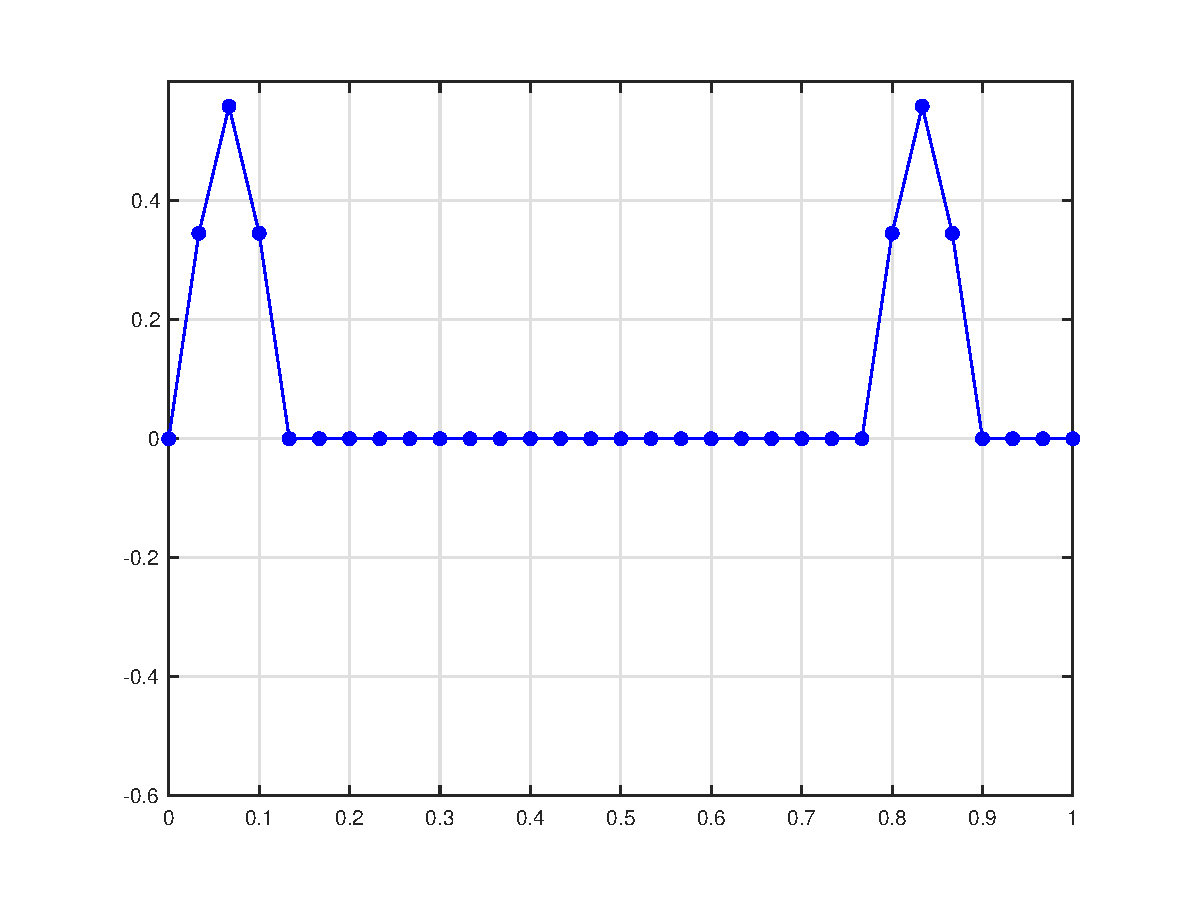
\includegraphics[width=0.33\textwidth]{plot1.eps}}}
    \subfloat[At the left boundary.]{\label{fig:leftBoundary}{ 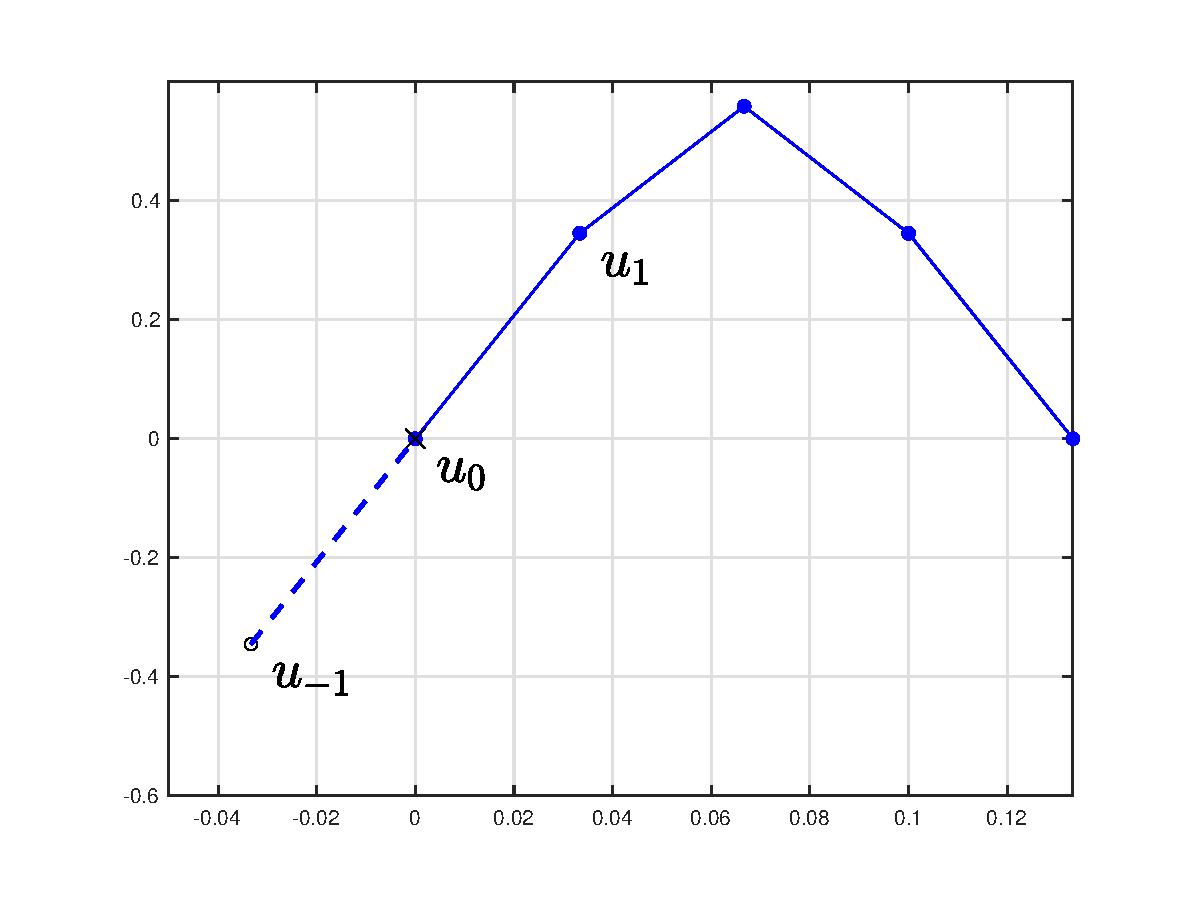
\includegraphics[width=0.33\textwidth]{plot2.eps}}}
    \subfloat[Curvature at the boundary (in this case at $u_0$) should be 0.]{\label{fig:boundaryCondition}{ 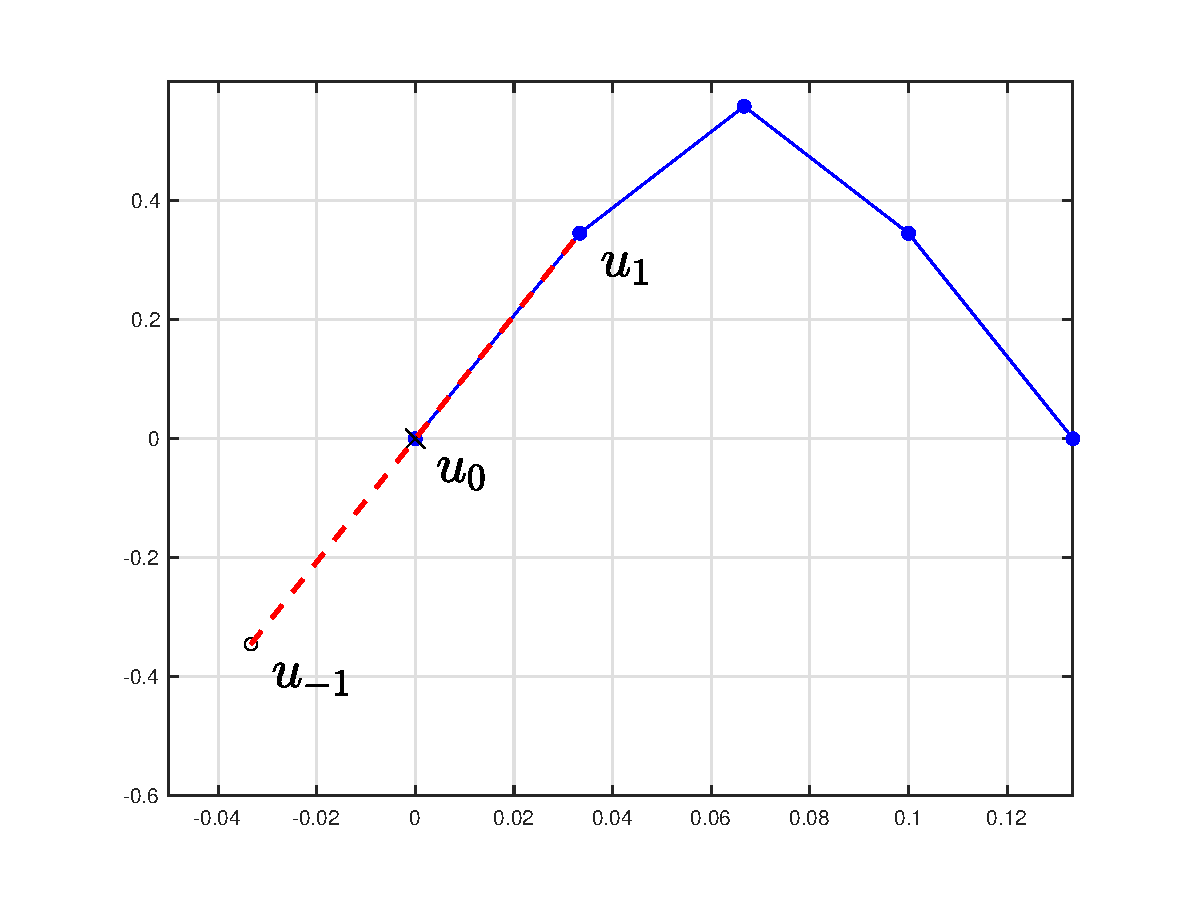
\includegraphics[width=0.33\textwidth]{plot3.eps}}}
    \caption{Case of grid point on boundary.}
\end{figure}

\begin{figure}[h]
\centerline{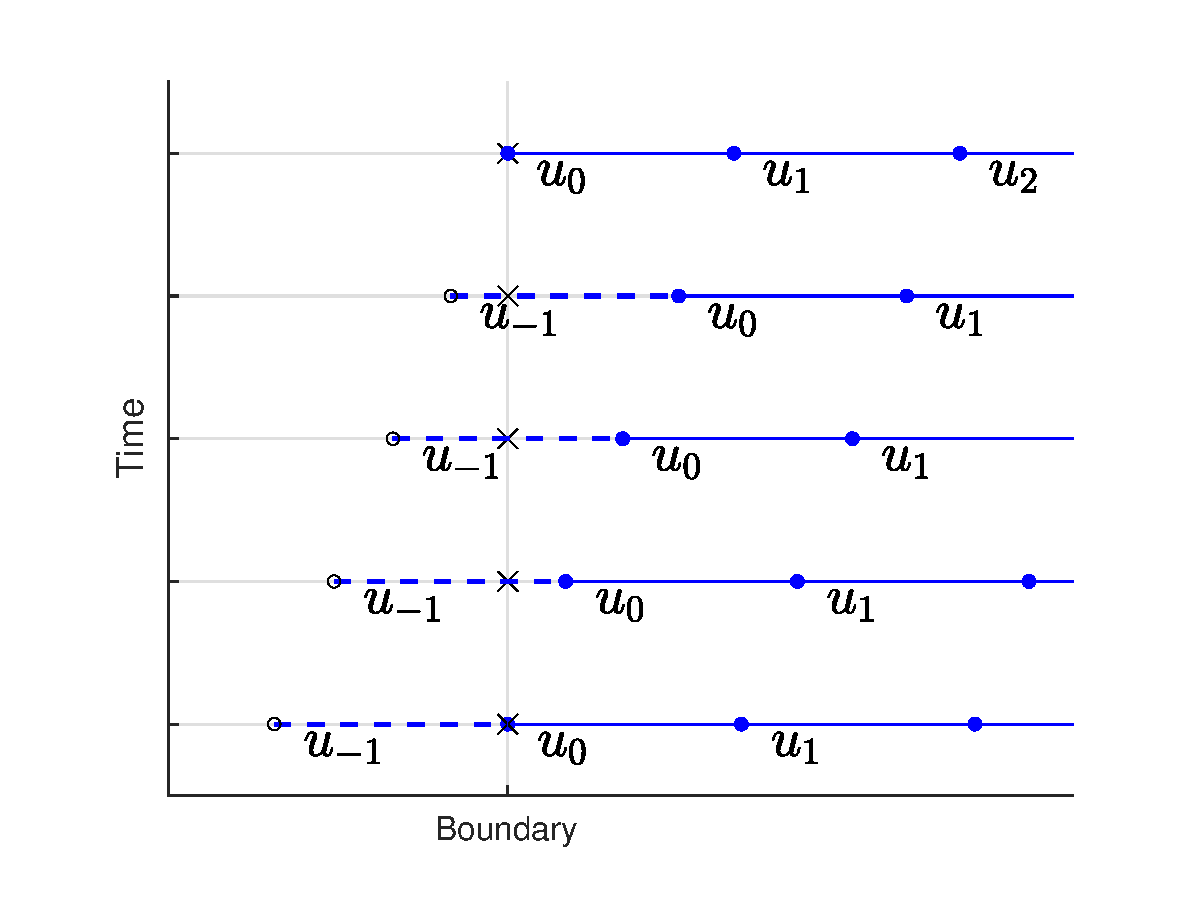
\includegraphics[width=0.6\columnwidth]{dynamic2.eps} }
\caption{\label{fig:dynamicGrid}{Grid changing over time.}}
\end{figure}

\subsection{Analogy with a real-life string}
Imagine detuning a real-life string by turning the tuning knob, we essentially change the value for tension $T$ in Eq. \eqref{eq:1Dwave}. If we imagine the tuning knob being at the nut (left boundary), more material will appear on that side when $T$ decreases, and vice versa. To make the transition to the finite-difference setting easier, imagine equidistant points drawn on this string in such a way that there is a point exactly at the nut and the bridge (i.e. at each boundary). Then, when decreasing the tension, the point at the nut will start moving towards the bridge. As a matter of fact, all points (except for the one at the bridge) will start moving towards the bridge! Effectively, we slowly decrease the space between the points which -- in a finite-difference setting -- is analogous to decreasing the grid spacing $h$ (see Figure \ref{fig:dynamicGrid} with time going from bottom to top). If we do this according to condition \eqref{eq:stabilityCondition}, we get the great side-effect of always satisfying this condition with equality, which means that we don't lose accuracy (or bandwidth). The issue left to solve now is to figure out what to do around the boundary. We continue by keeping in mind boundary condition \eqref{eq:boundaryCondition}.
% \begin{figure}[h]
% \centerline{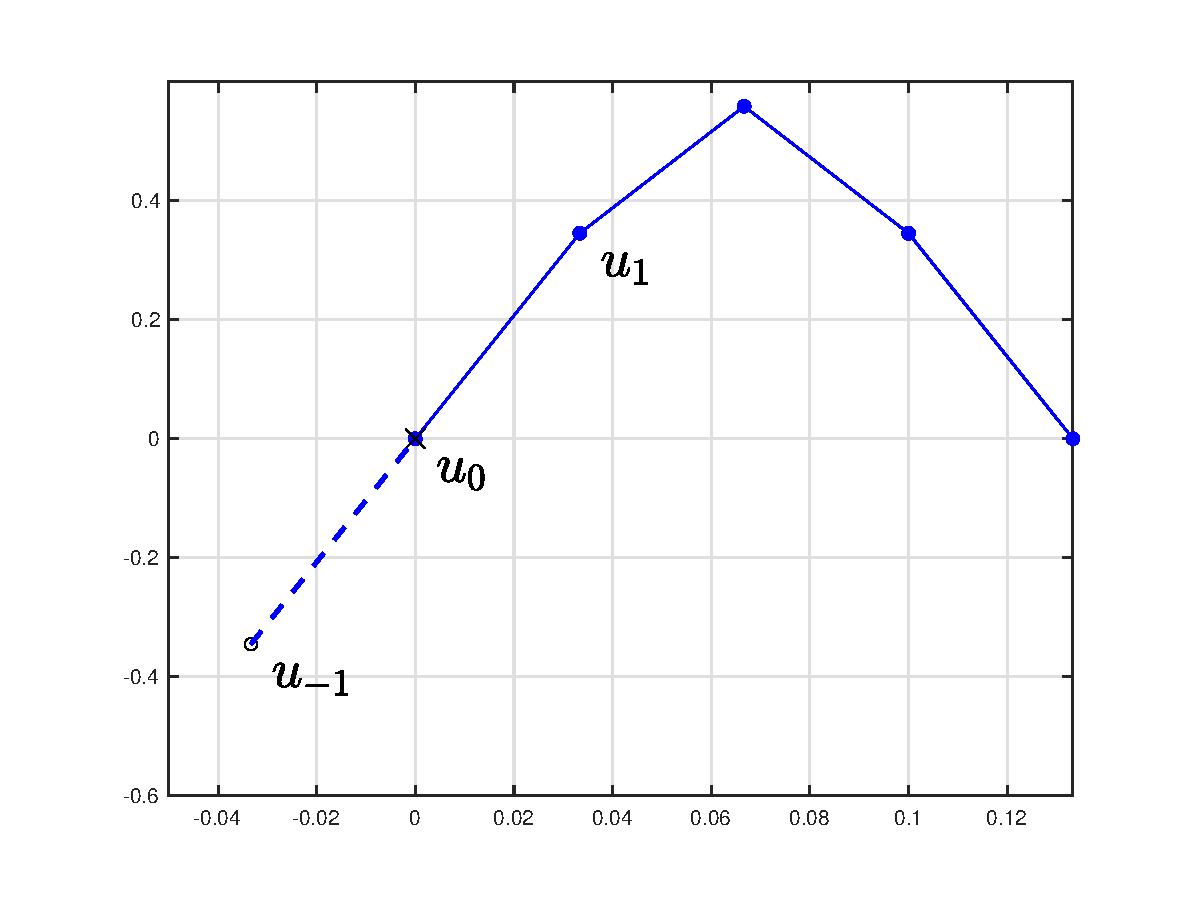
\includegraphics[width=0.6\columnwidth]{plot2.eps}}
% \caption{\label{fig:eta}{At the left boundary.}}
% \end{figure}

% \begin{figure}[h]
% \centerline{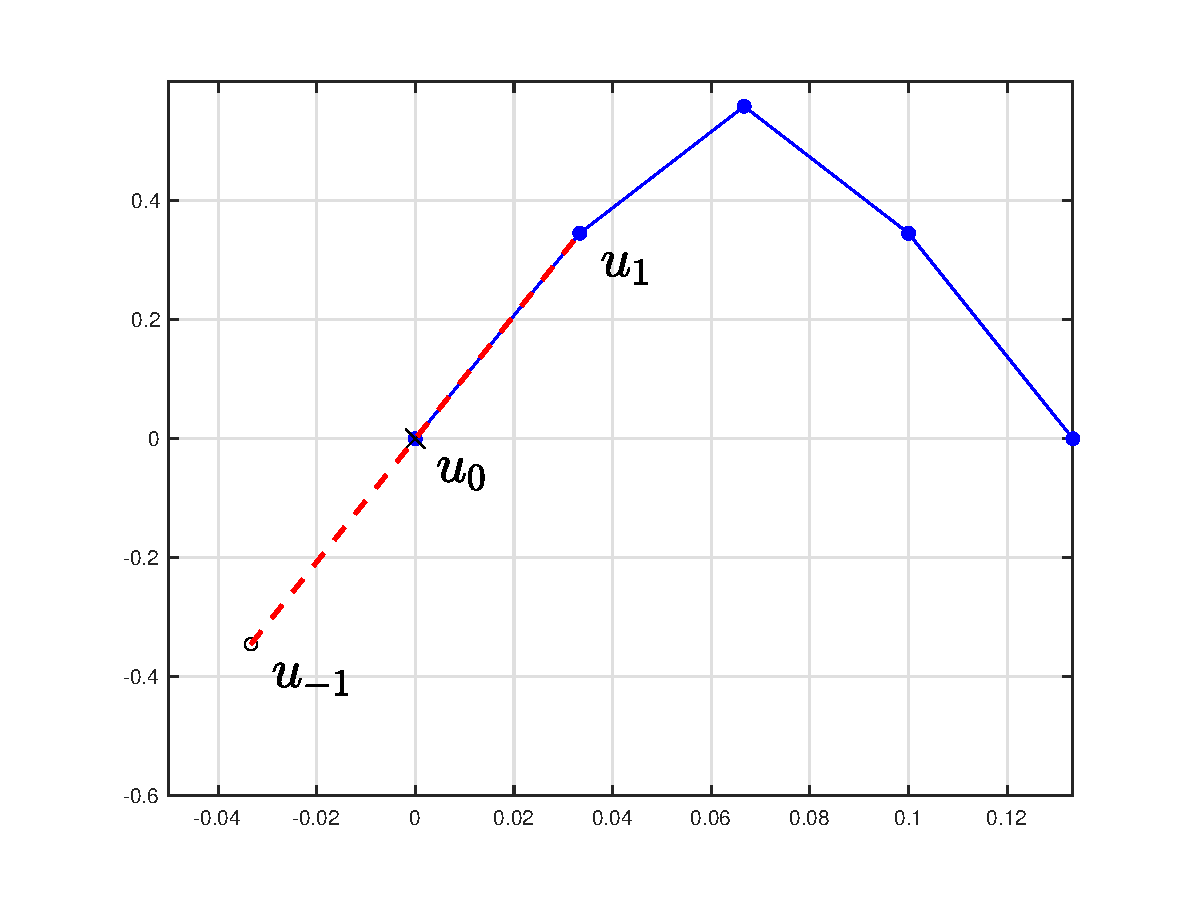
\includegraphics[width=0.6\columnwidth]{plot3.eps}}
% \caption{\label{fig:eta}{Boundary Condition. Curvature at $u_0$ needs to be 0.}}
% \end{figure}
\section{The Interpolated Boundary}
In this section, the location of a grid point $u_l$ along the string will be given by $x_l$. In the normal case, i.e., when the first grid point lays on the boundary ($x_0 = 0$), we can satisfy \eqref{eq:boundaryCondition} as follows:
\begin{equation}\label{eq:expandedBoundCond}
    \begin{aligned}
        &\delta_{xx}u_0 = 0\\
        &\frac{1}{h^2}(u_1 - 2u_0 + u_{-1}) = 0 \\[-13pt]
        \xLeftrightarrow{\mystrut\ u_0 = 0\ } \quad &u_{-1} = -u_1.
    \end{aligned}
\end{equation}
Applying this to an expanded version of Eq. \eqref{eq:1Dwave} is unnecessary, as we know that $u_0 = 0$ at all times, and therefore does not need to be updated. If $u_0$ doesn't lay on the boundary, however, we need to define and satisfy the boundary condition differently. Let's change the boundary condition to something more general to apply to a point $u_\text{B}$ which may or may not coincide with (or be equal to) $u_0$:
\begin{equation}\label{eq:generalBoundary}
        u_\text{B} = \delta_{xx}u_\text{B} = 0,
\end{equation}
where the location of the boundary along the string $x_\text{B} = 0$ at all times. Again, this condition states that the state as well as the curvature at the boundary needs to be 0. 

As $u_0$ is not necessarily $0$ (as it used to according to Eq. \eqref{eq:boundaryCondition}) we need to calculate it using the scheme in \eqref{eq:1Dwave}. We expand the scheme at $u_0$ and solve for $u_0^{n+1}$ as follows
\begin{equation}
    u_0^{n+1} = 2u_0^n - u_0^{n-1} + \lambda^2 (u_1^n - 2u_0^n+u_{-1}^n),
\end{equation}
where $\lambda = ck/h$. Now, we need a definition for virtual grid point $u_{-1}$, which we can obtain using the new boundary condition \eqref{eq:generalBoundary}.

In order to obtain a definition for the curvature at the boundary $\delta_{xx}u_\text{B}$, we need two points that are equally distant from the boundary. Starting from the virtual grid point $u_{-1}$ at the left side of the boundary, we can define some interpolated grid point $u_\text{I}$ with the same distance from the boundary as $u_{-1}$ (see Figure \ref{fig:dynamicBoundary} for a visualisation of this). 
\begin{figure}[h]
\centerline{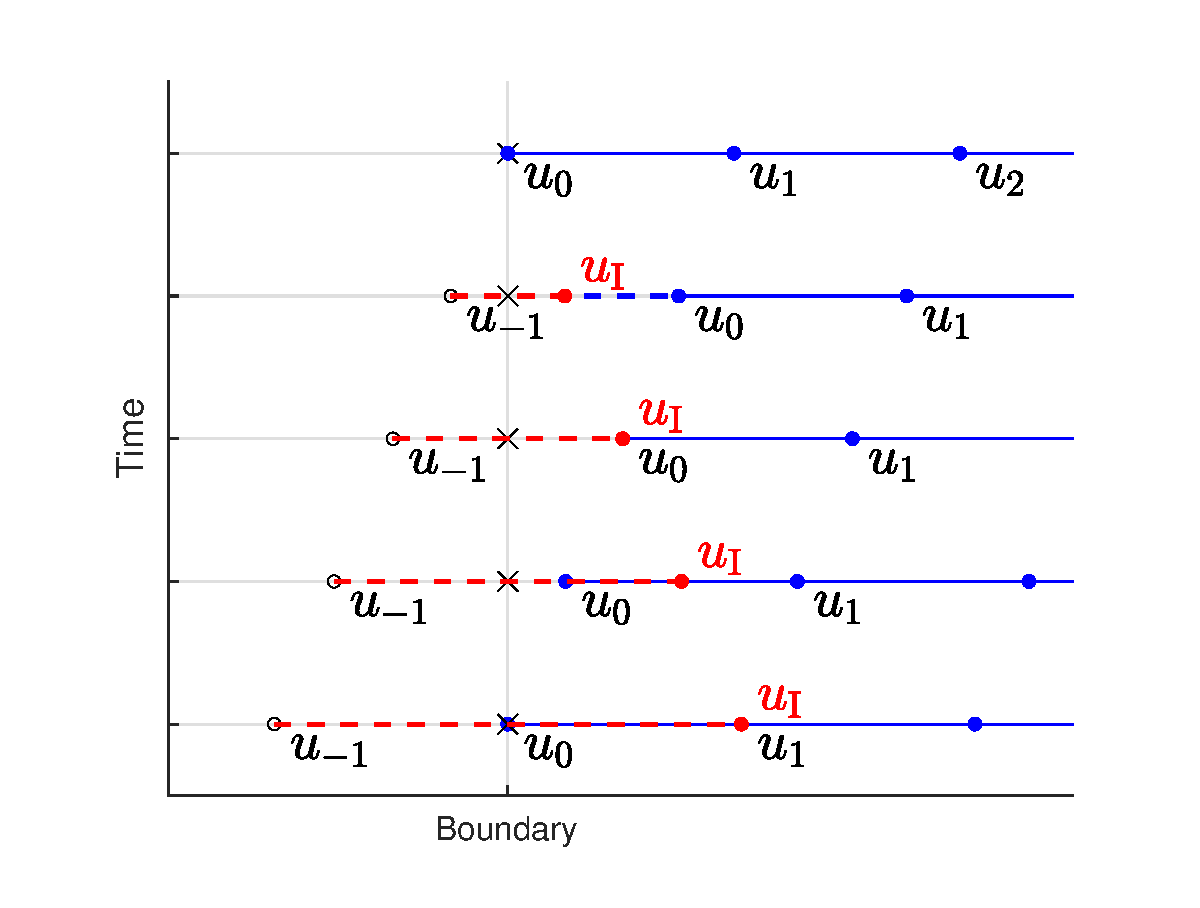
\includegraphics[width=0.6\columnwidth]{dynamicBoundaryDrawChange.eps}}
\caption{\label{fig:dynamicBoundary}{Boundary conditions at different values for $h$. Important to note is that the distance between $u_0$ and $u_{-1}$ always remains (the current) $h$. The distance between $u_{-1}$ and $u_\text{B}$ (and also $u_\text{I}$ and $u_\text{B}$) is defined as $h_\text{I}$. Then, from the location of $u_{-1}$, the location of $u_\text{I}$ (the interpolated point used to calculate the value of $u_{-1}$) is determined.}}
\end{figure}

This distance can be calculated using
\begin{equation}
    h_\text{I} = h - x_0,
\end{equation}
where $x_0$ is the location of $u_0$ along the string length. As $u_{-1}$ and $u_\text{I}$ have the same distance $h_\text{I}$ to the boundary and are at opposite sides, we can use these when expanding \eqref{eq:generalBoundary} and obtain a different definition for $u_{-1}$:
\begin{equation}
    \begin{aligned}
        &\delta_{xx}u_\text{B} = 0\\
        &\frac{1}{h_\text{I}^2} (u_\text{I} - 2u_\text{B} + u_{-1}) = 0\\[-13pt]
        \xLeftrightarrow{\mystrut\ u_\text{B} = 0\ } \quad & u_{-1} = - u_\text{I},
    \end{aligned}
\end{equation}
which is similar to condition \eqref{eq:expandedBoundCond}, but now using the interpolated state (or grid point) $u_\text{I}$. The last thing we need is a definition for this state which is currently done using linear interpolation. We do, however, need different definitions in the cases where $x_\text{I} > x_0$ (fourth instance from the top in Figure \ref{fig:dynamicBoundary}) and $x_\text{I} \leq x_0$ (second and third instance from the top in Figure \ref{fig:dynamicBoundary})
\begin{subequations}
    \begin{numcases}{}
        u_\text{I} = (1-\alpha) u_0 + \alpha u_1 \quad \text{where} \quad \alpha = \frac{h-2x_0}{h} &$ x_\text{I} > x_0$\label{eq:xiLarger}\\
        u_\text{I} = \underbrace{(1-\alpha) u_\text{B}}_{=0} + \alpha u_0 \quad \text{where} \quad \alpha = \frac{h_\text{I}}{x_0} &  $x_\text{I} \leq x_0$\label{eq:xiSmaller}
    \end{numcases}
\end{subequations}
% We can then use the distance of virtual grid point to $u_\text{B}$ to obtain a definition for it 

% Using $\lambda = ck/h$, expanding \eqref{eq:1Dwave} at the boundary and applying \eqref{eq:expandedBoundCond}:
% \begin{equation}
%     \begin{aligned}
%         u_0^{n+1} &= 2u_0^n - u_0^{n-1} + \lambda^2 (u_1^n-2u_0^n + u_{-1}^n)\\
%         \xLeftrightarrow{\text{Eq. \eqref{eq:expandedBoundCond}}}\quad u_0^{n+1} &= 2u_0^n - u_0^{n-1} + \lambda^2 (u_1^n-2u_0^n - u_1^n)\\
%         u_0^{n+1} &= 2u_0^n - u_0^{n-1} - 2\lambda^2 u_0^n
%     \end{aligned}
% \end{equation}
% we can see that the virtual grid point $u_{-1}$ essentially cancels out the effect that $u_1$ has on $u_0$.  
% satisfy the boundary condition: the curvature around the boundary needs to be $0$. 

\section{Energy}
We can get the energy of Eq. \eqref{eq:1Dwave} by first taking the inner product with respect to $\delta_{t\cdot}u$ like
\begin{equation}
    \delta_{t+}\mathfrak{h} = \rho A\langle \delta_{t\cdot}u, \delta_{tt}u\rangle_\mathcal{D} - T \langle \delta_{t\cdot}u,\delta_{xx}u\rangle_\mathcal{D} = 0,
\end{equation}
using integration by parts to get
\begin{equation}\label{eq:innerProd}
    \delta_{t+}\mathfrak{h} = \rho A\langle \delta_{t\cdot}u, \delta_{tt}u\rangle_\mathcal{D} + T \langle \delta_{t\cdot}\delta_{x+}u,\delta_{x+}u\rangle_{\underline{\mathcal{D}}} = \mathfrak{b},
\end{equation}
where boundary term
\begin{equation}
    \mathfrak{b} = T (\delta_{t\cdot}u_N)(\delta_{x+}u_N) - T(\delta_{t\cdot}u_0)(\underbrace{\delta_{x+}u_{-1}}_{\delta_{x-}u_0})\ .
\end{equation}
Expanding Eq. \eqref{eq:innerProd} yields,
\begin{equation}
    \delta_{t+}\mathfrak{h} = \rho A \sum_\mathcal{D}h(\delta_{t\cdot}u)(\delta_{tt}u) + T \sum_{\underline{\mathcal{D}}}h(\delta_{t\cdot}\delta_{x+}u)(\delta_{x+}u)
\end{equation}
Then, using the following identities  
\begin{subequations}
\begin{align}
    (\delta_{t\cdot}u)(\delta_{tt}u) &= \delta_{t+}\left(\frac{1}{2}(\delta_{t-}u)^2\right) \quad \text{and}\label{eq:identity1}\\
    (\delta_{t\cdot}u)u &= \delta_{t+}\left(\frac{1}{2}u e_{t-}u\right)\label{eq:identity2}
\end{align}
\end{subequations}
we can finally obtain the energy $\mathfrak{h}$:
\begin{gather}
        \mathfrak{h} = \mathfrak{t} + \mathfrak{v}\quad \text{where}\\
    \mathfrak{t} = \frac{\rho A}{2} \sum_{\mathcal{D}} h (\delta_{t-}u_l^n)^2 \quad \text{and} \quad \mathfrak{v} =  \frac{T}{2}\sum_{\underline{\mathcal{D}}}h (\delta_{x+}u_l^n)(\delta_{x+}u_l^{n-1})\nonumber
\end{gather}

In the case when $x_\text{I} \leq x_0$ (case \eqref{eq:xiSmaller}) we can find an energy definition for the left boundary:
\begin{equation}
    \begin{aligned}
        \delta_{t+}\mathfrak{h}_\text{l} &= T(\delta_{t\cdot}u_0)(\delta_{x-}u_0)\\
        &= \frac{T}{h}(\delta_{t\cdot}u_0)(u_0 - u_{-1})\\[-4pt]
        \xLeftrightarrow{\mystrut\ u_{-1} = -\alpha u_0\ } \quad & = \frac{T}{h}(\delta_{t\cdot}u_0)((1+\alpha)u_0)\\
        &= \frac{T(1+\alpha)}{h}(\delta_{t\cdot}u_0)u_0\\[-5pt]
        \xLeftrightarrow{\mystrut\ \text{Eq. \eqref{eq:identity2}}\ } \quad & = \frac{T(1+\alpha)}{h}\delta_{t+}\left(\frac{1}{2}u_0^nu_0^{n-1}\right)\\
        \mathfrak{h}_l &= \frac{T(1+\alpha)}{2h}u_0^nu_0^{n-1}
    \end{aligned}
\end{equation}
The next step will be to find the energy for case \eqref{eq:xiLarger} (if it exists....). Here follow the first steps:
\begin{equation}
    \begin{aligned}
        \delta_{t+}\mathfrak{h}_\text{l} &= T(\delta_{t\cdot}u_0)(\delta_{x-}u_0)\\
        &= \frac{T}{h}(\delta_{t\cdot}u_0)(u_0 - u_{-1})\\[-5pt]
        \xLeftrightarrow{\mystrut\ -u_{-1} = u_\text{I}\ \text{\&} \ \text{Eq. } \eqref{eq:xiLarger}\ } \quad & = \frac{T}{h}(\delta_{t\cdot}u_0)(u_0 + (1+\alpha) u_0 + \alpha u_1)\\
        &= \frac{T(2+\alpha)}{h}(\delta_{t\cdot}u_0)u_0 + \frac{T}{h}(\delta_{t\cdot}u_0)(\alpha u_1)\\[-5pt]
        \xLeftrightarrow{\mystrut\ \text{Eq. }\eqref{eq:identity2}\ } \quad &= \frac{T(2+\alpha)}{h}\delta_{t+}\left(\frac{1}{2}u_0^nu_0^{n-1}\right) + \underbrace{\frac{T}{h}(\delta_{t\cdot}u_0)(\alpha u_1)}_{\text{\SWcomment[The issue]}} 
    \end{aligned}
\end{equation}
\bibliographystyle{plain}
\bibliography{bibliography}

\appendix
\section{Note regarding issue when increasing $T$}\label{app:increasingT}
If we decrease $T$, the points smoothly enter the scheme without issues. However, in the opposite case when we increase $T$ (moving from top to bottom in Figure \ref{fig:dynamicGrid}), the string will already be moving at $u_0$ and continue moving due to its inertia (the $\rho A \delta_{tt}u$ term). In other words, even though we can satisfy the $\delta_{xx}u_0 = 0$ part of the boundary condition, $u_0=0$ is harder to satisfy. Something needs to be figured out for this..

\section{Alternative Approach: 1D-waves with connected free (Neumann) ends}
Another approach to changing the grid dynamically is to add / remove points in the center of the string rather than the boundaries (see Figure \ref{fig:twoFreeStrings}). I expect that doing this, rather than adding / removing points at the boundary, will allow for smoother changes when increasing $T$, i.e, when the amount of points decreases (see Appendix \ref{app:increasingT}). Consider a string, $u$ with $M_u = \text{ceil}(0.5/ck)$ (simply $M$ below for brevity) and $w$ with $M_w = \text{floor}(0.5/ck)$ points, i.e., half the number of points allowed by the stability condition $N$, plus one for overlap due to the combined $\text{ceil}$ $\text{floor}$ operations (will elaborate below). Then the following boundary conditions are imposed:
\begin{equation}\label{eq:halfStringBoundaryCond}
    \begin{aligned}
        u_0 = w_{M_w} &= 0,\quad \text{(Dirichlet)}\\
        \delta_{x\cdot}u_M = \delta_{x\cdot}w_0 &= 0\ \quad \text{(Neumann)}.
    \end{aligned}
\end{equation}

\begin{figure}[h]
\centerline{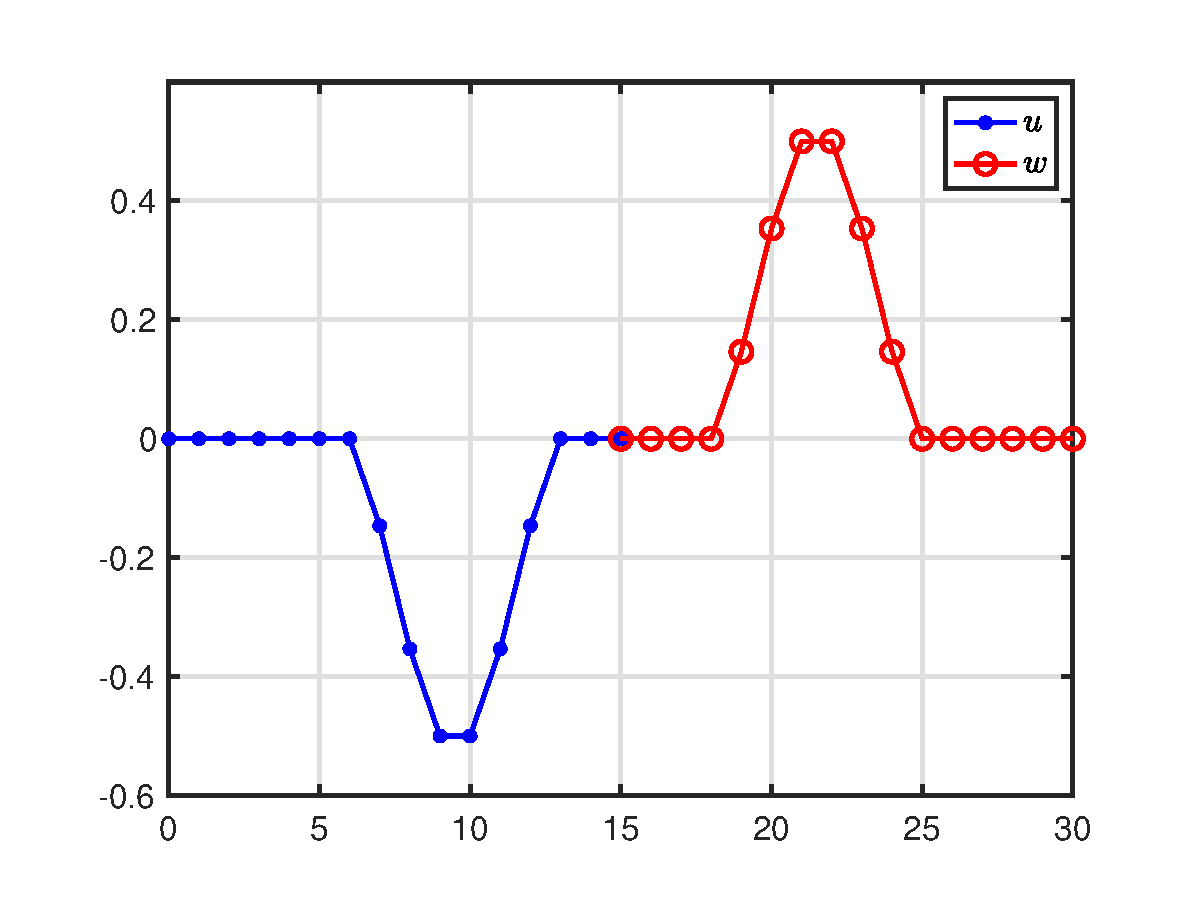
\includegraphics[width=0.6\columnwidth]{twoFreeStrings.eps} }
\caption{\label{fig:twoFreeStrings}{Two strings connected at one of their boundaries.}}
\end{figure}

\noindent Then we can connect $u_M$ and $w_0$ using a rigid connection, i.e.,
\begin{equation}\label{eq:rigid}
    u_M^n = w_0^n
\end{equation}
for all $n$. The system will now be
\begin{equation}
    \begin{cases}\label{eq:systemHalfStrings}
        \delta_{tt}u_l^n = c^2\delta_{xx}u_l^n + J(x_{u_M})F\\
        \delta_{tt}w_l^n = c^2\delta_{xx}w_l^n - J(x_{w_0})F
    \end{cases}
\end{equation}
where
\begin{equation}
    J(x_i) =
    \begin{cases}
        \frac{1}{h}, & l = l_i\\
        0,& \text{otherwise}
    \end{cases}
\end{equation}
If we expand the spatial derivative operators in \eqref{eq:systemHalfStrings} at $u_M$ and $w_0$ we get, recalling \eqref{eq:halfStringBoundaryCond}
\begin{equation}\label{eq:expandedSystem}
    \begin{cases}
        \delta_{tt}u_M^n = \frac{c^2}{h^2}(2u_{M-1}^n-2u_M^n) + \frac{1}{h}F\\
        \delta_{tt}w_0^n = \frac{c^2}{h^2}(2w_1^n-2w_0^n) - \frac{1}{h}F.
    \end{cases}
\end{equation}
Because \eqref{eq:rigid} is true we also know that $\delta_{tt}u_M^n = \delta_{tt}w_0^n$ for all $n$. We can then calculate $F$, by setting the equations in \eqref{eq:systemHalfStrings} equal to each other:

% \begin{equation}
% \begin{aligned}
%     c^2\delta_{xx}u_M^n + \frac{1}{h} F &= c^2\delta_{xx}w_0^n - \frac{1}{h} F\\
%     \frac{c^2}{h^2}(u_{M-1}^n-2u_M^n+u_{M+1}^n) + \frac{1}{h} F &= \frac{c^2}{h^2}(w_{-1}^n-2w_0^n+w_1^n) - \frac{1}{h} F
% \end{aligned}\nonumber
% \end{equation}

% \noindent Knowing through \eqref{eq:halfStringBoundaryCond} that $u_{M+1} = u_{M-1}$ and $w_{-1} = w_1$   yields
\begin{align}
     \frac{c^2}{h^2}(2u_{M-1}^n-2u_M^n) + \frac{1}{h} F&= 
     \frac{c^2}{h^2}(2w_1^n-2w_0^n) - \frac{1}{h} F\\
    \frac{2}{h}F &= \frac{c^2}{h^2}(2w_1^n - 2u_{M-1}^n)\nonumber\\
    F &= h \frac{c^2}{h^2}(w_1^n - u_{M-1}^n)
\end{align}
Filling this into \eqref{eq:expandedSystem} after expansion of the second-time derivative yields
\begin{subequations}\label{eq:resultOneConnectedPoint}
\begin{numcases}{}
    u^{n+1}_M = 2u_M^n - u_n^{n-1} + \lambda^2(u_{M-1}^n-2u_M^n+w_1^n)\label{eq:resultOneConnectedPoint1}\\
    w^{n+1}_0 = 2w_0^n - w_0^{n-1} + \lambda^2(u_{M-1}^n-2w_0^n+w_1^n)\label{eq:resultOneConnectedPoint2}
\end{numcases}
\end{subequations}
which, (again, recalling \eqref{eq:rigid}) are indeed equivalent expressions for the connected point. Here, $w_1$ in the first expression acts as virtual grid point $u_{M+1}^n$ and $u_{M-1}^n$ as virtual grid point $w_{-1}^n$. So essentially, to connect the two strings we add a state of one string to the update of the other.

\subsection{Changing the grid}
The previous is an exact solution to the problem when the stability condition is satisfied with equality, i.e, when $1/ck$ is an integer. If we then want to change the grid spacing according to $h=ck$ we leave the locations of the outer boundaries ($u_0$ and $w_{M_w}$) fixed and move the rest of the points towards their respective outer boundary (see Figure \ref{fig:interpolated}). 

We now continue with the idea of adding a state of one string in the update of the other. When the stability condition is not satisfied with equality -- and thus the points of the strings don't overlap -- we use linear interpolator $I_1$. This results in,
\begin{align}
    u_{M+1}^n &= I_1(x_{u_{M+1}})w_l^n = (1-\alpha)w_1^n + \alpha w_0^n\\
    w_{-1}^n &= I_1(x_{w_{-1}})u_l^n = (1-\alpha)u_{M-1}^n + \alpha u_M^n
\end{align}
where
\begin{equation}
    \alpha = \frac{x_{w_0} - x_{u_M}}{h},
\end{equation}
and grid-point locations $x_{u_{M+1}}$ and $w_{-1}$. Note that when $h$ changes the connected points start to move away from each other.
\begin{figure}[h]
    \centering
    \subfloat[When $h$ changes.]{\label{fig:interpolatedFull}{ 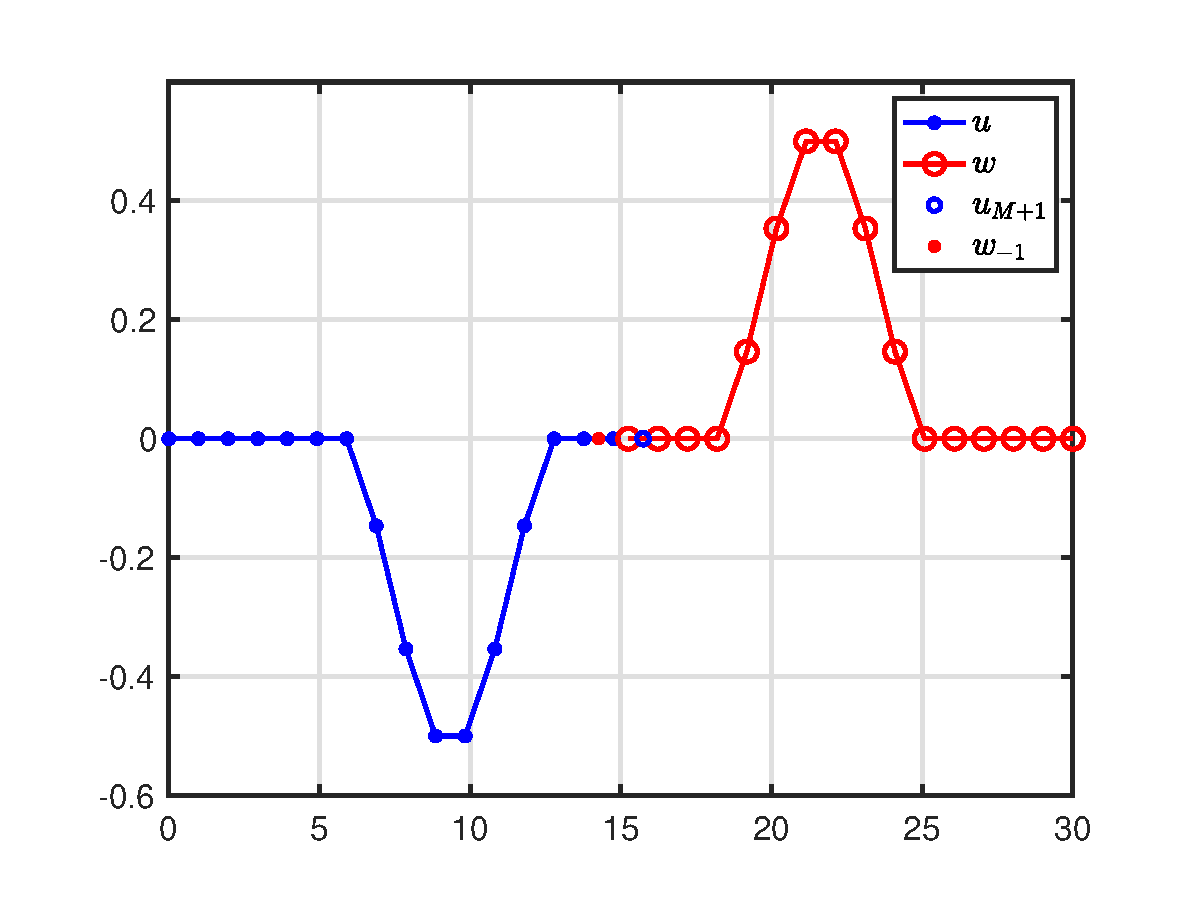
\includegraphics[width=0.5\textwidth]{twoFreeStringsInterpolatedFull.eps}}}
    \subfloat[Zoomed]{\label{fig:interpolatedZoom}{ 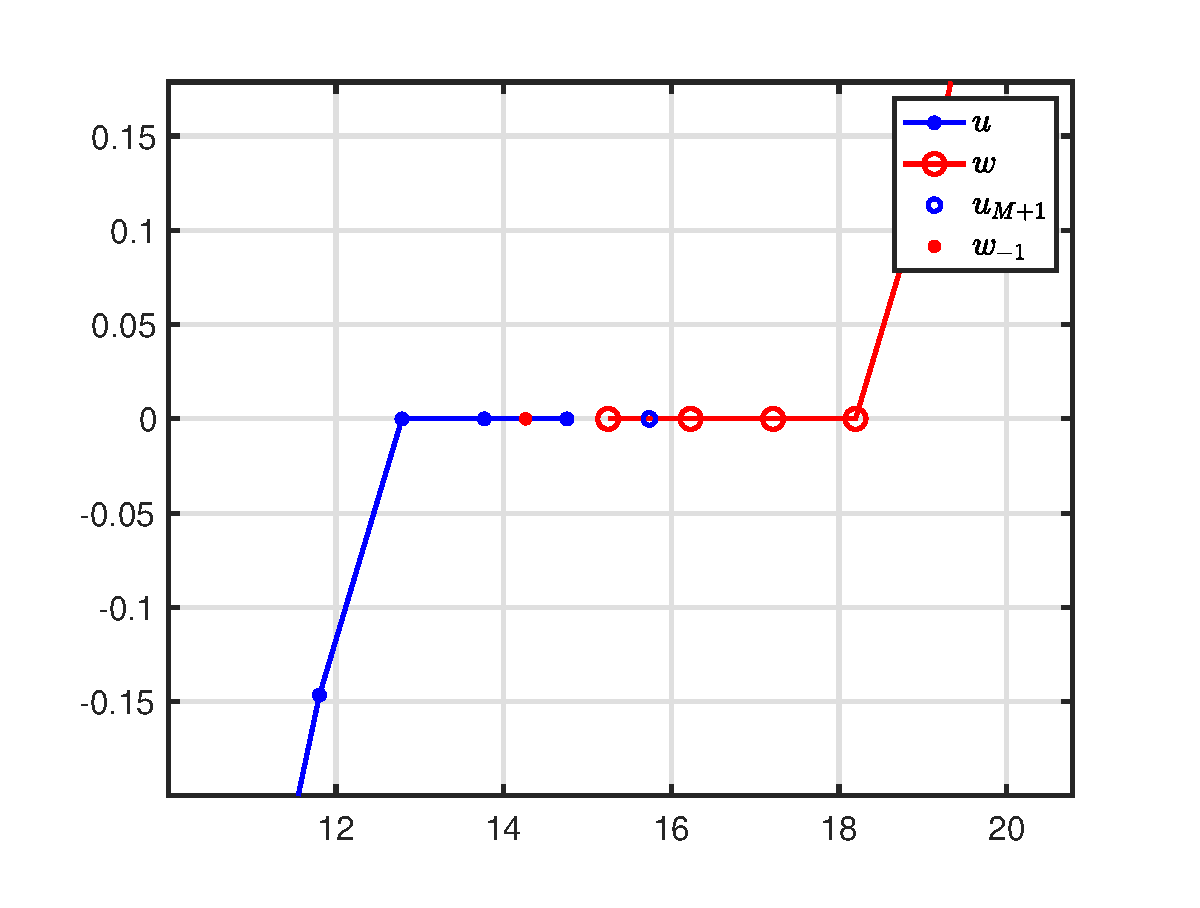
\includegraphics[width=0.5\textwidth]{twoFreeStringsInterpolated.eps}}}
    \caption{}\label{fig:interpolated}
\end{figure}
%
Then, when the boundary points surpass with the virtual points (i.e. $x_{u_M} \leq x_{w_{-1}}$ and $x_{u_{M+1}} \leq x_{w_0}$) we alternate between adding / removing a point to the right side of $u$ and the left side of $w$.
\begin{equation}\label{eq:addingRemovingPoints}
    \begin{cases}
        \begin{cases}\mathbf{u}^n = [\mathbf{u}^n, I(x_{u_{M+1}})\mathbf{w}^n]^T & \text{if $N^n$ is odd}\\
        \mathbf{w}^n = [I(x_{w_{-1}})\mathbf{u}^n, \mathbf{w}^n]^T & \text{if $N^n$ is even}
        \end{cases} & \text{if } N^n > N^{n-1} \text{ (adding a point)}\\
        \\
        \begin{cases}
        \mathbf{u}^n = [u_0^n, u_1^n ..., u_{M-1}^n]^T & \text{if $N^n$ is even} \\
         \mathbf{w}^n = [w_1^n, w_2^n ..., w_{M_w}^n]^T & \text{if $N^n$ is odd} 
        \end{cases} &\text{if } N^n < N^{n-1} \text{ (removing a point)}
        % u^{n-1} = [u^{n-1}, I(x_{u_{M+1}})w^{n-1}];
    \end{cases}
\end{equation}
The interpolator used is
\begin{equation}
    I = \begin{bmatrix} -\frac{\alpha(\alpha+1)}{(\alpha+2)(\alpha+3)} &\frac{2\alpha}{\alpha+2} &\frac{2}{\alpha+2} 
    &-\frac{2\alpha}{(\alpha+3)(\alpha+2)}
    \end{bmatrix},
\end{equation}
with
\begin{equation}
    \alpha = \frac{x_{w_0} - (x_{u_M} + h)}{h}\ .
\end{equation}
Even though subjective listening confirmed that the sound is smooth when adding / removing points using linear interpolation, the expected fundamental frequency ($f_0 \approx c/2$) was slightly too high when interpolation needed to happen. Instead of a linear, we will use cubic interpolator $I_3$ according to 
% \begin{equation}\label{eq:connectionInterpol}
%     \begin{aligned}
%         u_{M+1}^n = I_3(x_{u_{M+1}})w_l^n &= \frac{\alpha(\alpha - 1)(\alpha - 2)}{-6} w_2^n + \frac{(\alpha - 1)(\alpha + 1)(\alpha - 2)}{2}w_1^n \\
%         &+ \frac{\alpha(\alpha + 1)(\alpha - 2)}{-2}w_0^n + \frac{\alpha(\alpha + 1)(\alpha - 1)}{6} w_{-1}^n\\
%         w_{-1}^n = I_3(x_{w_{-1}})u_l^n &= \frac{\alpha(\alpha - 1)(\alpha - 2)}{-6} u_{M-2}^n + \frac{(\alpha - 1)(\alpha + 1)(\alpha - 2)}{2}u_{M-1}^n \\
%         &+ \frac{\alpha(\alpha + 1)(\alpha - 2)}{-2}u_M^n + \frac{\alpha(\alpha + 1)(\alpha - 1)}{6} u_{M+1}^n.
%     \end{aligned}
% \end{equation}

\begin{equation}\label{eq:connectionInterpol}
    \begin{aligned}
        u_{M+1}^n &= I_3(x_{u_{M+1}})w_l^n &&= \alpha_\text{I}w_2^n + \beta_\text{I}w_1^n + \gamma_\text{I}w_0^n + \delta_\text{I} w_{-1}^n\\
        w_{-1}^n &= I_3(x_{w_{-1}})u_l^n &&=\alpha_\text{I} u_{M-2}^n + \beta_\text{I}u_{M-1}^n+ \gamma_\text{I}u_M^n + \delta_\text{I} u_{M+1}^n.
    \end{aligned}
\end{equation}
where
\begin{gather*}
    \alpha_\text{I} = \frac{\alpha(\alpha - 1)(\alpha - 2)}{-6}, \quad \beta_\text{I} = \frac{(\alpha - 1)(\alpha + 1)(\alpha - 2)}{2},\\
    \gamma_\text{I} = \frac{\alpha(\alpha + 1)(\alpha - 2)}{-2}, \quad \text{and} \quad\delta_\text{I} = \frac{\alpha(\alpha + 1)(\alpha - 1)}{6}\,.
\end{gather*}
We can solve for $u_{M+1}^n$ and $w_{-1}^n$ by treating \eqref{eq:connectionInterpol} as a linear system of equations
\begin{equation}\label{eq:matSolution}
    \begin{bmatrix}
    u_{M+1}^n \\
    w_{-1}^n
    \end{bmatrix}
    =
    \mathbf{A}^{-1}
    \mathbf{v},
\end{equation}
where
% \begin{equation}\nonumber
%     \mathbf{A} = \begin{bmatrix}
%          1 & -\frac{\alpha(\alpha + 1)(\alpha - 1)}{6} \\
%          -\frac{\alpha(\alpha + 1)(\alpha - 1)}{6} & 1
%     \end{bmatrix},
% \end{equation}
% and
% \begin{equation}\nonumber
%     \mathbf{v} = \begin{bmatrix}
%     \frac{\alpha(\alpha - 1)(\alpha - 2)}{-6} w_2^n+ \frac{(\alpha - 1)(\alpha + 1)(\alpha - 2)}{2}w_1^n + \frac{\alpha(\alpha + 1)(\alpha - 2)}{-2}w_0^n \\
%     \frac{\alpha(\alpha - 1)(\alpha - 2)}{-6} u_{M-2}^n + \frac{(\alpha - 1)(\alpha + 1)(\alpha - 2)}{2}u_{M-1}^n + \frac{\alpha(\alpha + 1)(\alpha - 2)}{-2}u_{M}^n
%     \end{bmatrix}.
% \end{equation}

\begin{equation}\label{eq:Av}
    \mathbf{A}
    =
     \begin{bmatrix}
         1 & -\delta_\text{I} \\
         -\delta_\text{I} & 1
    \end{bmatrix} \quad \text{and} \quad \mathbf{v} = \begin{bmatrix}
    \alpha_\text{I} w_2^n+ \beta_\text{I}w_1^n + \gamma_\text{I}w_0^n \\
    \alpha_\text{I} u_{M-2}^n + \beta_\text{I}u_{M-1}^n + \gamma_\text{I} u_{M}^n
    \end{bmatrix}.
\end{equation}

Using cubic interpolation gives us the expected fundamental frequency for any wave speed. This can be proven using modal analysis, described in the following section.

\subsection{Modal Analysis}
It is possible to write the complete system in matrix form as
\begin{equation}
    \mathbf{U}^{n+1} = \mathbf{B}\mathbf{U}^n - \mathbf{U}^{n-1}
\end{equation}
where \begin{equation}
\mathbf{U}^n = \begin{bmatrix}
\mathbf{u}^n\\
\mathbf{w}^n
\end{bmatrix}.
\end{equation}
%
If $\alpha = 0$ and the outer boundaries of the system ($u_0$ and $w_{M_w}$) are excluded from $\mathbf{U}$, $\mathbf{B}$ looks like
\begin{equation}
    \mathbf{B} = 2\mathbf{I} + \lambda^2 \begin{bmatrix}[cccccc|cccccc]
        &-2 & 1 & & & & & & & & & \\
        &1 & -2 & 1 & & & & & & & & \\
        &  & \ddots  &\ddots & \ddots & & & & 0 & & & \\
       & & & 1 & -2 & 1 &  & & & & & \\
       && & & 1 & -2 & 0 & 1 & & & & \\ \cline{2-11}
      & & & & 1 & 0 &-2 & 1 & & & & \\
         & & & & & &1 & -2 & 1 & & & \\
         & & & 0 & & &  & \ddots  &\ddots & \ddots & & \\
        & & & & & & & & 1 & -2 & 1 & \\
        & & & & & & & & & 1 & -2 & 
    \end{bmatrix}
\end{equation}
The $1$'s in the top-right and bottom-left quadrant show the interaction between $\mathbf{u}$ and $\mathbf{w}$ as shown in \eqref{eq:resultOneConnectedPoint}. In other words, $u_M^n$ is calculated using $w_1^n$ and $w_0^n$ using $u_{M-1}^n$.

We can change $\mathbf{B}$ to include linear interpolation using (focusing only on the middle of the matrix)
% \begin{equation}
%     \mathbf{B}_1 = 2\mathbf{I} + \lambda^2 \begin{bmatrix}[cccccc|cccccc]
%         &-2 & 1 & & & & & & & & & \\
%         &1 & -2 & 1 & & & & & & & & \\
%         &  & \ddots  &\ddots & \ddots & & & & 0 & & & \\
%       & & & 1 & -2 & 1 &  & & & & & \\
%       && & & 1 & -2 & \alpha & (1-\alpha) & & & & \\ \cline{2-11}
%       & & & & (1-\alpha) & \alpha &-2 & 1 & & & & \\
%          & & & & & &1 & -2 & 1 & & & \\
%          & & & 0 & & &  & \ddots  &\ddots & \ddots & & \\
%         & & & & & & & & 1 & -2 & 1 & \\
%         & & & & & & & & & 1 & -2 & 
%     \end{bmatrix}
% \end{equation}

\begin{equation}
    \mathbf{B}_1 = 2\mathbf{I} + \lambda^2 \begin{bmatrix}[cccc|cccc]
     & \ddots  &\ddots & & & & 0 & \\
       & 1 & -2 & 1 & & & & \\
      & & 1 & -2 & \alpha & (1-\alpha) & \\ \cline{2-7}
      & & (1-\alpha) & \alpha &-2 & 1 & & \\
         & & & &1 & -2 & 1  \\
         & 0 & &  &  &\ddots & \ddots &
    \end{bmatrix}
\end{equation}

Cubic interpolation is slightly trickier but still possible. Renaming $\mathbf{A}^{-1}$ from Eq. \eqref{eq:Av} to $\mathbf{A}^\text{i}$ and writing out \eqref{eq:matSolution} yields
\begin{align}
    u_{M+1}^n = \mathbf{A}^\text{i}_{1, 1}\begin{bmatrix}
   \gamma_\text{I} & \beta_\text{I} & \alpha_\text{I}
    \end{bmatrix} \begin{bmatrix}
   w_0^n & w_1^n &w_2^n
    \end{bmatrix}^T + \mathbf{A}^\text{i}_{1, 2}\begin{bmatrix}
   \alpha_\text{I} & \beta_\text{I} & \gamma_\text{I}
    \end{bmatrix} \begin{bmatrix}
   u_{M-2}^n & u_{M-1}^n &u_M^n
    \end{bmatrix}^T\\
    w_{-1}^n = \mathbf{A}^\text{i}_{2, 1}\begin{bmatrix}
   \gamma_\text{I} & \beta_\text{I} & \alpha_\text{I}
    \end{bmatrix} \begin{bmatrix}
   w_0^n & w_1^n &w_2^n
    \end{bmatrix}^T + \mathbf{A}^\text{i}_{2, 2}\begin{bmatrix}
   \alpha_\text{I} & \beta_\text{I} & \gamma_\text{I}
    \end{bmatrix} \begin{bmatrix}
   u_{M-2}^n & u_{M-1}^n &u_M^n
    \end{bmatrix}^T
\end{align}
Recalling Eq. \eqref{eq:resultOneConnectedPoint1} where $w_1^n$ acts as virtual grid point $u_{M+1}^n$ and Eq. \eqref{eq:resultOneConnectedPoint2}
we can use this to insert the solution from \eqref{eq:matSolution} into $\mathbf{B}$ according to

\begin{equation}
    \mathbf{B}_3 = 2\mathbf{I} + \lambda^2 \begin{bmatrix}[cccc|cccc]
     & \ddots  &\ddots & & & & 0 & \\
       & 1 & -2 & 1 & & & & \\
      & \mathbf{A}_{1, 2}^\text{i}\alpha_\text{I} &\mathbf{A}_{1, 2}^\text{i}\beta_\text{I} + 1 &\mathbf{A}_{1, 2}^\text{i}\gamma_\text{I} -2 & \mathbf{A}_{1, 1}^\text{i}\gamma_\text{I} & \mathbf{A}_{1, 1}^\text{i}\beta_\text{I}& \mathbf{A}_{1, 1}^\text{i}\alpha_\text{I}\\ \cline{2-7}
      &\mathbf{A}_{2, 2}^\text{i}\alpha_\text{I} &\mathbf{A}_{2, 2}^\text{i}\beta_\text{I}&\mathbf{A}_{2, 2}^\text{i}\gamma_\text{I} & \mathbf{A}^\text{i}_{2,1}\gamma_\text{I}-2 & \mathbf{A}^\text{i}_{2,1}\beta_\text{I}+ 1 &\mathbf{A}_{2, 1}^\text{i}\alpha_\text{I} & \\
         & & & &1 & -2 & 1  \\
         & 0 & &  &  &\ddots & \ddots &
    \end{bmatrix}
\end{equation}
The modal frequencies (eigenfrequencies) of the system can then be calculated using the following formula \cite[p. 174]{Bilbao2009}
\begin{equation}
    f_p = \frac{1}{2\pi k}\cos^{-1}\left(\frac{1}{2}\text{eig}_p(\mathbf{B})\right).
\end{equation}

\subsubsection{Deciding the location of adding / removing points}
Until now we have only looked at adding / removing points at the center of the string as in Eq. \eqref{eq:addingRemovingPoints}. The results for this can be found in Figure \ref{fig:modesAddInCenter}. Multiple things can be seen from this figure: 
\begin{itemize}
    \item At every integer $N$, there are $N-1$ modes (related to the number of moving points at that point) that are integer multiples of the fundamental. Due to the extra point used for overlap, an extra mode arises between the lower and the upper half of the harmonics. If the system is excited on an integer $N$, this extra mode will not be excited due to the constraint of a rigid connection. 
    \item Modal crossings: 
\end{itemize}

\begin{figure}[h]
\centerline{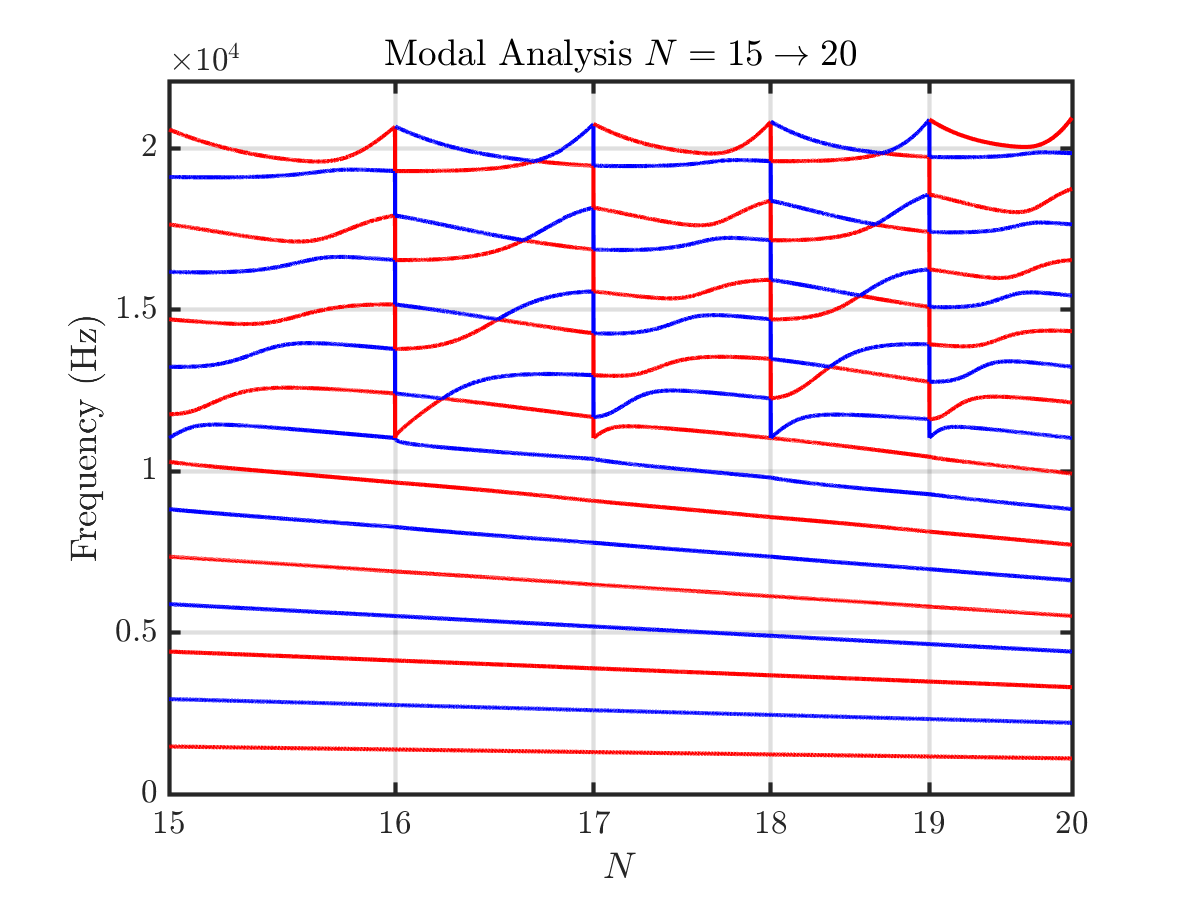
\includegraphics[width=0.6\columnwidth]{modesAddPointsInCenter.eps} }
\caption{\label{fig:modesAddInCenter}{Modal analysis of 1D wave going linearly from $c = 2940$ m/s ($N=15$) to $c =2205$ m/s ($N=20$).}}
\end{figure}

\subsection{Stiff string}
To prove that this technique also works with more complicated schemes, we can apply the above to the stiff string with the following scheme
\begin{equation}
    \delta_{tt}u = c^2\delta_{xx}u - \kappa^2\delta_{xxxx}u
\end{equation}
where $\kappa = \sqrt{EI/\rho A}$ with Young's modulus $E$ and moment of inertia $I$. The difference with the 1D-wave equation is the stiffness term containing a fourth order spatial derivative. This requires an extra virtual grid point to be calculated at the boundaries. For the outer boundaries we choose simply supported conditions according to
\begin{equation}
    u_0 = w_{M_w} = \delta_{xx}u_0 =  \delta_{xx}w_{M_w} = 0.
\end{equation}
The points needed at the other boundaries are calculated below. 

We start by (again) connecting $u_{M}^n$ and $w_0^n$ using a rigid connection using \eqref{eq:rigid} yielding the following system:
\begin{equation}
    \begin{cases}
        \delta_{tt}u_l^n = c^2\delta_{xx}u_l^n-\kappa^2\delta_{xxxx}u_l^n + J(x_{u_M})F\\
        \delta_{tt}w_l^n = c^2\delta_{xx}w_l^n -\kappa^2\delta_{xxxx}w_l^n - J(x_{w_0})F.
    \end{cases} 
\end{equation}
If we expand the spatial derivative operators and using the concept of weight ratio due to the overlap (see Appendix \ref{app:overlap}) we get
\begin{equation}\label{eq:systemHalfStiffStrings}
    \begin{cases}
        \delta_{tt}u_M^n = \frac{c^2}{h^2}(2u_{M-1}^n-u_M^n)-\frac{\kappa^2}{h^4}(2u_{M-2}^n - 8u_{M-1}^2+6u_M^n) + \frac{1}{h}F\\
        \delta_{tt}w_0^n = \frac{c^2}{h^2}(2w_1^n-w_0^n)-\frac{\kappa^2}{h^4}(2w_2^n - 8w_1^2+6w_0^n) - \frac{1}{h}F.
    \end{cases} 
\end{equation}
Again, because \eqref{eq:rigid} is true, $\delta_{tt}u_M = \delta_{tt}w_0$ and by setting the equations in \eqref{eq:systemHalfStiffStrings} equal to each other we can solve for $F$
\begin{gather}
    \frac{c^2}{h^2}(2u_{M-1}^n- 2u_M^n)-\frac{\kappa^2}{h^4}(2u_{M-2}^n - 8u_{M-1}^n + 6 u_M^n) + \frac{1}{h}F =  \nonumber\\
    \frac{c^2}{h^2}(2w_1^n - 2w_0^n) -\frac{\kappa^2}{h^4}(2w_2^n - 8w_1^n + 6w_0^n) - \frac{1}{h}F\nonumber\\
    \frac{2}{h}F = \frac{c^2}{h^2}(2w_1^n - 2w_0^n-2u_{M-1}^n+2u_M^n)-\frac{\kappa^2}{h^4}(2w_2^n - 8w_1^n + 6w_0^n - 2u_{M-2}^n + 8u_{M-1}^n - 6u_M^n)\nonumber\\
    F = h\frac{c^2}{h^2}(w_1^n-u_{M-1}^n)-h\frac{\kappa^2}{h^4}(w_2^n-4w_1^n+4u_{M-1}^n-u_{M-2}^n).
\end{gather}
If we add this to the respective equations in \eqref{eq:systemHalfStiffStrings} and expand the acceleration term to get the following updates
\begin{equation}\label{eq:systemHalfStiffStrings}
    \begin{cases}
        u_M^{n+1} = 2u_M^n - u_M^{n-1}+ \lambda^2(u_{M-1}^n-2u_M^n+w_1^n)-\mu^2(u_{M-2}^n - 4u_{M-1}^2+6u_M^n-4w_1^n+w_2^n)\\
        w_0^{n+1} = 2w_0^n - w_0^{n-1}+ \lambda^2(u_{M-1}^n-2w_0^n+w_1^n)-\mu^2(u_{M-2}^n - 4u_{M-1}^2 + 6w_0^n - 4w_1^2 + w_2^n),
    \end{cases} 
\end{equation}
which are (again) equivalent expressions for the connected point. 

\SWcomment[Along the same lines\footnote{might have to prove something here}] we can find updates for $u_{M-1}^n$ and $w_1^n$, which -- through the fourth-order spatial derivative -- are now also affected by the state of the other string:
\begin{equation}\label{eq:systemHalfStiffStrings}
    \begin{cases}
        u_{M-1}^{n+1} = 2u_{M-1}^n - u_{M-1}^{n-1}+ \lambda^2(u_{M-2}^n-2u_{M-1}^n+u_M^n)-\mu^2(u_{M-3}^n - 4u_{M-2}^n+6u_{M-1}^n-4u_M^n+w_1^n)\\
        w_1^{n+1} = 2w_1^n - w_1^{n-1}+ \lambda^2(w_0^n-2w_1^n+w_2^n)-\mu^2(u_{M-1}^n - 4w_0^n + 6w_1^n - 4w_2^n + w_3^n).
    \end{cases} 
\end{equation}
\section{Adding an overlap}\label{app:overlap}
Another, slightly trickier, setup could be that the left string has an extra point at its right side to cause some overlap. This might come in handy later if we want to interpolate the forces between the strings for better quality. We can then apply two rigid connections to the overlapping points
\begin{equation}\label{eq:doubleRigid}
    \begin{aligned}
    u_{M-1}^n &= w_0^n,\\
    u_M^n &= w_1^n.
    \end{aligned}
\end{equation}
See Figure \ref{fig:overlap} for clarification. 

\begin{figure}[h]
    \centering
    \subfloat[Overlapped points.]{\label{fig:overlapFull}{ 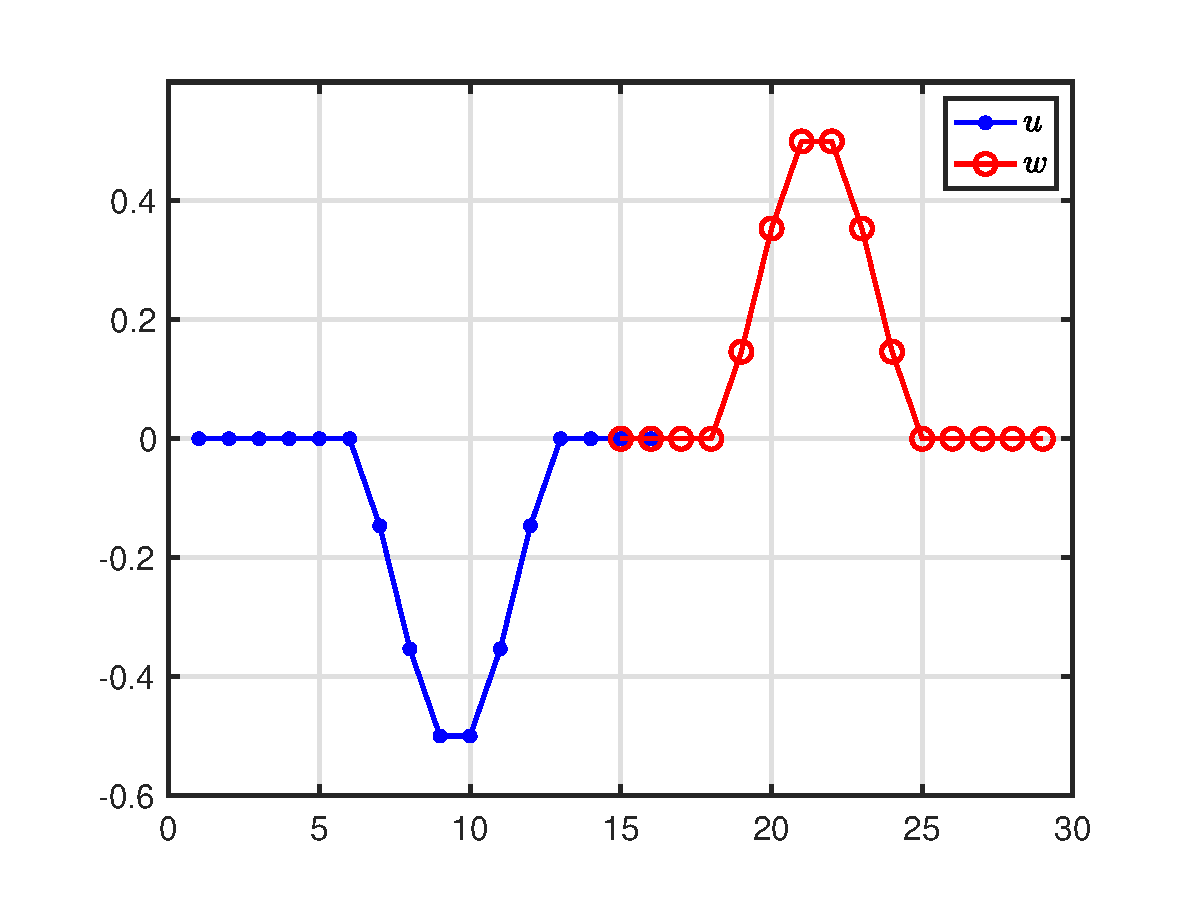
\includegraphics[width=0.5\textwidth]{twoStringsOverlap.eps}}}
    \subfloat[Zoomed. Note that the overlapping points should always have the same state, but they have been pulled apart for clarity.]{\label{fig:overlapZoom}{ 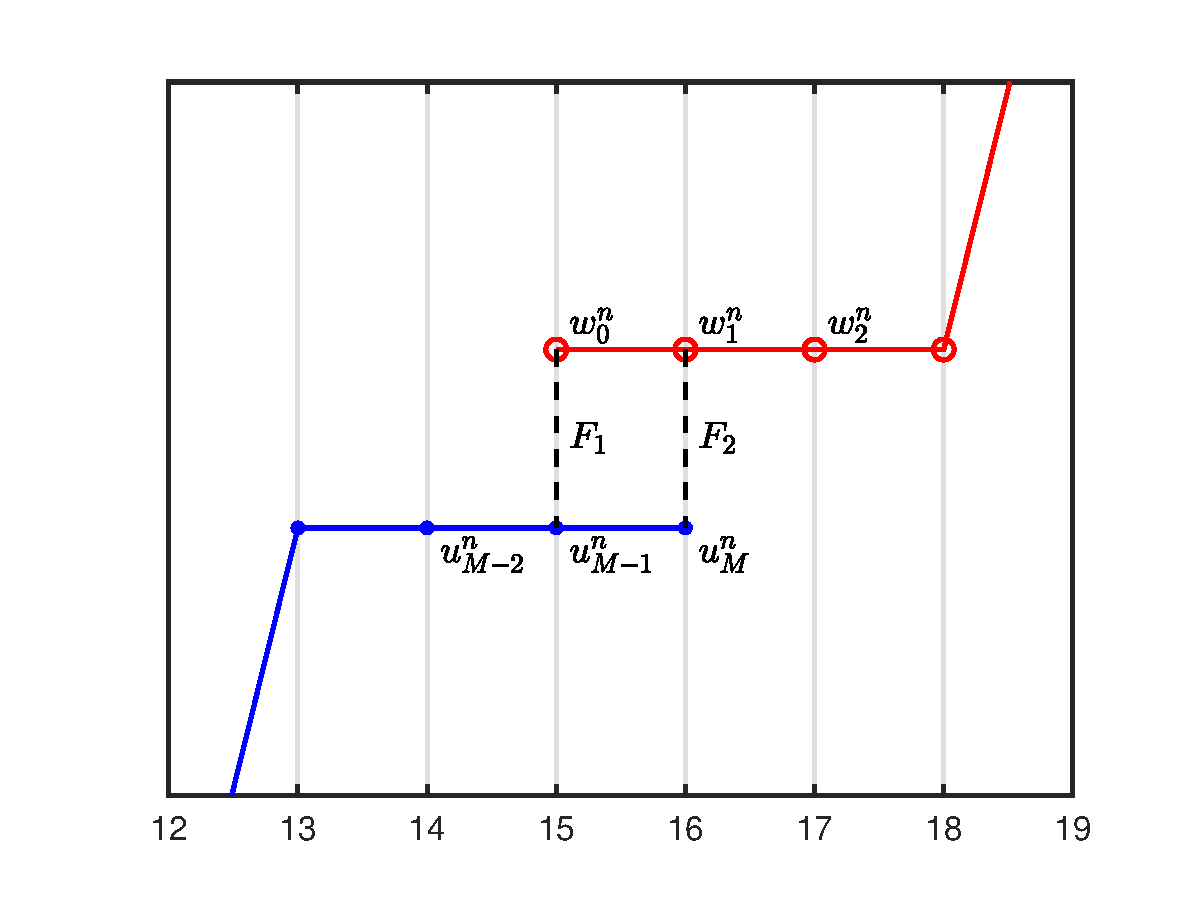
\includegraphics[width=0.5\textwidth]{overlapForces.eps}}}
    \caption{}\label{fig:overlap}
\end{figure}

As an overlap happens, the string is ``heavier" at this point if we keep the same physical parameters. However, in reality, the string is equally heavy everywhere. As shown in Figure \ref{fig:overlapZoom}, the overlapping points ($u_{M-1}^n, u_{M}^n, w_0^n$ and $w_1^n$) have to be made twice as light as their non-overlapping counterparts. From their perspective, $u_{M-2}^n$ and $w_2^n$ are twice as heavy when compared to themselves. Imagine changing the material density of these to double of what they usually are. This will change the wave speed according to:
\begin{equation}
    c^2 = T/\rho A \quad \xRightarrow[]{\ 2\rho\ }\quad c^2 = T/2\rho A \quad \Rightarrow \quad 2c^2 = T/\rho A.
\end{equation}

For the overlapping points, we will now have the following update equations
\begin{equation}\label{eq:updateOverlap}
    \begin{cases}
        u_{M-1}^{n+1} = 2u_{M-1}^n - u_{M-1}^{n-1} + \lambda^2 (2u_{M-2}^n - 2u_{M-1}^n + u_{M}^n) + \frac{k^2}{h}F_1\\
        u_{M}^{n+1} = 2u_{M}^n - u_{M}^{n-1} + \lambda^2 (u_{M-1}^n - 2u_M^n) + \frac{k^2}{h}F_2\\
        w_0^{n+1} = 2w_0^n-w_0^{n-1} + \lambda^2 (w_1^n-2w_0^n) - \frac{k^2}{h}F_1\\
        w_1^{n+1} = 2w_1^n-w_1^{n-1} + \lambda^2 (w_0^n-2w_1^n+2w_2^n) - \frac{k^2}{h}F_2
    \end{cases}
\end{equation}
\SWcomment[One would think that some scaling also needs to happen for $u_{M-1}^n$ in the update equation for $u_{M-2}^{n+1}$ and $w_1^n$ in $w_2^n$, but as we will see shortly, this is not necessary.]
This concept of a weight ratio also automatically happened in the previous case because of the Neumann boundary condition.

Recalling \eqref{eq:doubleRigid}, we can then solve for $F_1$ and $F_2$ in the same way as before. 

\begin{align}
    2u_{M-1}^n - u_{M-1}^{n-1} + \lambda^2(2u_{M-2}^n-2u_{M-1}^n + u_{M}^n) + \frac{k^2}{h} F_1 &=
    2w_0^n - w_0^{n-1} + \lambda^2(w_1^n-2w_0^n) - \frac{k^2}{h} F_1\nonumber\\
    \frac{2k^2}{h}F_1 &= \lambda^2(- 2u_{M-2}^n)\nonumber\\
    F_1 &= -h \frac{c^2}{h^2}(u_{M-2}^n)
\end{align}
and 
\begin{align}
    2u_M^n - u_M^{n-1} + \lambda^2(u_{M-1}^n-2u_M^n) + \frac{k^2}{h} F_2 &=
    2w_1^n - w_1^{n-1} + \lambda^2(w_0^n-2w_1^n+2w_2^n) - \frac{k^2}{h} F_2\nonumber\\
    \frac{2k^2}{h}F_2 &= \lambda^2(2w_2^n)\nonumber\\
    F_2 &= h \frac{c^2}{h^2}(w_2^n).
\end{align}

When filled into the update equations in \eqref{eq:updateOverlap} we get 
\begin{equation}\label{eq:updateOverlap}
    \begin{cases}
        u_{M-1}^{n+1} = 2u_{M-1}^n - u_{M-1}^{n-1} + \lambda^2 (u_{M-2}^n - 2u_{M-1}^n + u_{M}^n)\\
        u_{M}^{n+1} = 2u_{M}^n - u_{M}^{n-1} + \lambda^2 (u_{M-1}^n - 2u_M^n + w_2^n)\\
        w_0^{n+1} = 2w_0^n-w_0^{n-1} + \lambda^2 (w_1^n-2w_0^n+u_{M-2}^n)\\
        w_1^{n+1} = 2w_1^n-w_1^{n-1} + \lambda^2 (w_0^n-2w_1^n+w_2^n).
    \end{cases}
\end{equation}
Here, similarly to \eqref{eq:resultOneConnectedPoint}, $w_2^n$ and $u_{M-2}^n$ in the updates for $u_M^{n+1}$ and $w_0^{n+1}$ respectively act as virtual grid points.
Now we can also see why as scaling for overlapping points $u_{N-1}^n$ and $w_1^n$ in the updates for $u_{M-2}^{n+1}$ and $w_2^{n+1}$ are not necessary.

\subsubsection{Preliminary tests..}
...show instability...

\subsection{Energy}
For the kinetic energy, we now have to add a scaling with $0.5$, not only to the last point, but also to the rest of the overlapping ones:
\begin{align}
    \mathfrak{t}_u &= \sum_{l=0}^{M-2}   h(\delta_{t-}u_l^n)^2 + \frac{h}{2}(\delta_{t-}u_{M-1}^n)^2 + \frac{h}{2}(\delta_{t-}u_M^n)^2\\
    \mathfrak{t}_w &= \sum_{l=2}^{M}h(\delta_{t-}w_l^n)^2 + \frac{h}{2}(\delta_{t-}w_0^n)^2 + \frac{h}{2}(\delta_{t-}w_1^n)^2
\end{align}
\begin{align}
    \mathfrak{v}_u &= \frac{c^2}{2}\sum_{l=0}^{M-2} h(\delta_{x+}u_l^n)(\delta_{x+}u_l^{n-1}) + c^2\frac{h}{4} (\delta_{x+}u_{M-1}^n)(\delta_{x+}u_{M-1}^{n-1})\\
    \mathfrak{v}_w &= \frac{c^2}{2}\sum_{l=1}^{M-1} h(\delta_{x+}w_l^n)(\delta_{x+}w_l^{n-1}) + c^2\frac{h}{4} (\delta_{x+}w_0^n)(\delta_{x+}w_0^{n-1})
\end{align}

\section{Dirichlet Condition (Stefan)}

Consider a domain of length $L$, and grid spacing $h = ck$ (so, right at the Courant limit). Set $N = floor(L/h)$. Set the grid locations to be
\begin{equation}
x_{0} = 0,\quad x_{1} = h,\quad\hdots,\quad x_{N-1} = (N-1)h, \quad x_{N} = L = (N+\alpha)h
\end{equation}
where $0\leq \alpha\leq 1$. The final grid point lies directly on the boundary. 

Under Dirichlet conditions, we set $u_{0} = 0$ and $u_{N} = 0$. The Laplacian takes the form\footnote{\SWcomment[$\frac{2}{\alpha+1} = \frac{2}{\alpha+\SWcomment[2]}+\frac{2}{(\alpha+2)(\alpha+1)}$]}
\begin{eqnarray}
    \delta_{xx}u_{1}&=& \frac{1}{h^2}\left(u_{2}-2u_{1}\right)\\
    \delta_{xx}u_{l} &=& \frac{1}{h^2}\left(u_{l+1}-2u_{l}+u_{l-1}\right)\qquad 2\leq l\leq N-2\\
    \delta_{xx}u_{N-1} &=& \frac{1}{h^2}\left(\frac{2}{\alpha+2}u_{N-2}-\frac{2}{\alpha+1}u_{N-1}\right)\label{eq:uNmin1}
\end{eqnarray}
and thus, in matrix form, 
\begin{equation}
{\bf D}_{xx} = \frac{1}{h^2} 
    \begin{bmatrix}
    -2 & 1 & & &\\
    1 & -2 & 1 & &\\
     & \ddots & \ddots & \ddots & \\
     && 1 & -2 & 1\\
     &&& \frac{2}{\alpha+2} & -\frac{2}{\alpha+1}\\
    \end{bmatrix}
\end{equation}
The scheme, as a whole, then looks like
\begin{equation}
    \delta_{tt}{\bf u}^{n} = c^2{\bf D}_{xx}{\bf u}^{n}
\end{equation}
Define the matrix ${\bf P}$ as
\begin{equation}
    {\bf P} = {\rm diag}\left(1,1,\hdots,\frac{\alpha+2}{2}\right)
\end{equation}
Then ${\bf P D}_{xx}$ is now symmetric. 

Left-multiplying the scheme by ${\bf P}$ and then taking the inner product with $\delta_{t\cdot}{\bf u}$ then gives a conserved energy. Notice that this reduces to the usual case when $\alpha = 0$. 

\subsection{Taylor series expansion (Silvin)}
To get to the coefficients for $u_{N-2}$ and $u_{N-1}$ in \eqref{eq:uNmin1} we use a Taylor series expansion around the grid point $N-1$. To start, it is easiest to assume an expansion around 0 and then apply it to a different location. 

Suppose we have three grid locations $x_{-1} = -h, x_0 = 0$ and $x_1 = h (\alpha + 1)$ and their function values $u_{-1}, u_0$ and $u_1$. We then want to find an approximation $L = \frac{\partial^2 u}{\partial x^2} + O(h)$ (where $O(h)$ describes the order of the error) of the form
%
\begin{equation}\label{eq:formL}
    L = a_{-1}u_{-1} + a_0 u_0 + a_1 u_1
\end{equation}
%
where the coefficients $a_{-1}, a_0$ and $a_1$ depend on $\alpha$. \SWcomment[I suppose in the regular case ($\alpha = 0$) the coefficients end up being $a_{-1} = 1/h^2$, $a_0 = -2/h^2$ and $a_1 = 1/h^2$.] To find these coefficients we perform a Taylor series expansion. First we need to assume for a continuous function $u(x)$ that $u_{-1} = u(x_{-1}), u_0 = u(x_0)$ and $u_1 = u(x_1)$. We can then approximate this function $u$ around location $x_0 (=0)$ as 
\begin{equation}\label{eq:taylor}
    u(x) = u(0) + \frac{du(0)}{dx}x + \frac{1}{2}\frac{d^2u(0)}{dx^2}x^2 + O(x^3).
\end{equation}
Here, $O(x^3)$ describes the order of the error (or the collective error term with order of $x^3$).

We can then fill in the values of $x_{-1}$ and $x_1$ above ($u(x_0) = u(0)$) to get
\begin{align}
    u(-h) &= u(0) + \frac{du(0)}{dx}(-h) + \frac{1}{2}\frac{d^2u(0)}{dx^2}(-h)^2 + O(h^3)\nonumber\\
    &= u(0) - h \frac{du(0)}{dx} + \frac{h^2}{2}\frac{d^2u(0)}{dx^2} + O(h^3),
\end{align}
and 
\begin{align}
    u(h(\alpha+1)) &= u(0) + \frac{du(0)}{dx}(h(\alpha+1)) + \frac{1}{2}\frac{d^2u(0)}{dx^2}(h(\alpha+1))^2 + O(h^3)\nonumber\\
    &= u(0) + h(\alpha+1) \frac{du(0)}{dx} + \frac{h^2(\alpha+1)^2}{2}\frac{d^2u(0)}{dx^2} + O(h^3).
\end{align}
The goal is then to solve for $\frac{d^2u(0)}{dx^2}$ as this is what we want to approximate in \eqref{eq:1Dwave}. We want to get rid of the first-order derivative term so we can perform the following addition
\begin{align}
    u(-h) + \frac{u(h(\alpha+1))}{\alpha+1} &= \left(1+\frac{1}{\alpha+1}\right)u(0) + \left(-h + \frac{h(\alpha+1)}{\alpha + 1}\right)\frac{du(0)}{dx} + \left(\frac{h^2}{2} + \frac{h^2(\alpha+1)^2}{2(\alpha+1)}\right)\frac{d^2u(0)}{dx^2}+ O(h^3)\nonumber\\
    \frac{(\alpha+1)u(-h) + u(h(\alpha+1))}{\alpha+1}&= \left(\frac{\alpha + 2}{\alpha + 1}\right) u(0) + \left(\frac{h^2 + h^2(\alpha+1)}{2}\right)\frac{d^2u(0)}{dx^2}+ O(h^3)\nonumber\\
    \!\!\!\!\!\!\!\!\!\!\!\!\!\!\!\!\!\!\!\!\!\!\!\!\!\!\!\!\!\!\!\!\!\!\!\frac{(\alpha+1)u(-h) - (\alpha+2)u(0)+ u(h(\alpha+1))}{\alpha+1}&= \left(\frac{h^2(\alpha+2)}{2}\right)\frac{d^2u(0)}{dx^2}+ O(h^3)\nonumber\\
    L = \frac{d^2u(0)}{dx^2} + O(h) &= \frac{2((\alpha+1)u(-h) - (\alpha+2) u(0) + u(h(\alpha+1)))}{h^2(\alpha+2)(\alpha+1)}.
\end{align}
Note that due to a division with $h^2$ the order of the error is $O(h)$ rather than $O(h^3)$.
The coefficients in \eqref{eq:formL} are then as follows:
\begin{equation}
    a_{-1} = \frac{2}{h^2(\alpha+2)}, \quad a_0 = -\frac{2}{h^2(\alpha+1)}, \quad \text{and} \quad a_1 = \frac{2}{h^2(\alpha+2)(\alpha+1)}.
\end{equation}
% \subsubsection{Using forward and backward approximations for the first order derivatives}
% Then, we need to approximate the derivatives in \eqref{eq:taylor}. When $x = x_{-1}$, the first derivative is defined as (backwards)
% \begin{equation}
%     \frac{du(0)}{dx} \approx \frac{u(0) - u(-h)}{h} = \frac{u_0 - u_{-1}}{h}\ ,
% \end{equation}
% and when $x = x_{1}$ it is (forwards)
% \begin{equation}
%     \frac{du(0)}{dx} \approx \frac{u(h(\alpha+1)) - u(0)}{h(\alpha+1)} = \frac{u_1 - u_{0}}{h(\alpha + 1)}\ .
% \end{equation}
% From these we can get a definition of the second derivative
% \begin{align}
%     \frac{d^2u(0)}{dx^2} &= \frac{\frac{u_1 - u_0}{h(\alpha+1)} - \frac{u_0 - u_{-1}}{h}}{\frac{h(\alpha+1) + h}{2}}\nonumber\\
%     &= \frac{\left(\frac{2(u_1-u_0-(\alpha+1)u_0+(\alpha+1)u_{-1})}{h(\alpha+1)}\right)}{h(\alpha+2)}\nonumber\\
%     &= \frac{2(u_1-(\alpha+2)u_0+(\alpha+1)u_{-1})}{h^2(\alpha+2)(\alpha+1)}\label{eq:secondOrderTaylor}
% \end{align}

% we can fill in the values of $x_{-1}$ and $x_1$ above ($u(x_0) = u_0$) to get
% \begin{align}
%     u(-h) &= u_0 + \frac{u_0 - u_{-1}}{h}(-h) + \frac{1}{2} \frac{2(u_1-(\alpha+2)u_0+(\alpha+1)u_{-1})}{h^2(\alpha+2)(\alpha+1)} (-h)^2\nonumber\\
%     &= u_{-1} + \frac{u_1-(\alpha+2)u_0+(\alpha+1)u_{-1}}{(\alpha+2)(\alpha+1)}\nonumber\\
% &= \left(1+\frac{1}{\alpha+2}\right)u_{-1} - \frac{1}{\alpha+1} u_0 + \frac{1}{(\alpha+2)(\alpha+1)}u_1,
% \end{align}
% and
% \begin{align}
%     u(h(\alpha+1)) &= u_0 + \frac{u_1-u_0}{h}(h(\alpha+1)) + \frac{1}{2} \frac{2(u_1-(\alpha+2)u_0+(\alpha+1)u_{-1})}{h^2(\alpha+2)(\alpha+1)} (h(\alpha+1))^2\nonumber\\
%     &= u_0 + (\alpha + 1) (u_1 - u_0) + \frac{(\alpha+1)(u_1-(\alpha+2)u_0+(\alpha+1)u_{-1})}{\alpha + 2}\nonumber\\
%     &= \frac{(\alpha + 1)^2}{\alpha + 2} u_{-1} - (2(\alpha+1) - 1)u_0 + \left((\alpha+1) + \frac{\alpha+1}{\alpha+2}\right)u_1.
% \end{align}
% We can then use these terms to approximate the second derivative
% \begin{align}
%     L &= \frac{1}{h^2}\big[u(-h)-2u(0)+u(h(\alpha+1))\big]\\
%     &= \frac{1}{h^2}\left[\left(\frac{(\alpha+2) + 1 + (\alpha+1)^2}{\alpha+2}\right)u_{-1} - \left(\frac{1}{\alpha+1}+ 2(\alpha+1) - 1 + 2\right)u_0 + \left(\frac{1 + (\alpha+2)(\alpha+1)^2 + (\alpha+1)^2}{(\alpha+2)(\alpha+1)}\right)u_1\right]
% \end{align}
% \SWcomment[However, here it seems that if $\alpha = 0$, the approximation becomes $L = \frac{1}{h^2}(2u_{-1} - 4u_0 + 2u_1)$, i.e., twice what it is supposed to be..]
% \subsubsection{Using the centered approximation for the first order derivative}
% Instead, we can approximate the first derivative with a centered approximation:
% \begin{equation}
%     \frac{du(0)}{dx} \approx \frac{u(h(\alpha+1) - u(-h))}{h + h(\alpha+1)} = \frac{u_1 - u_{-1}}{h(\alpha + 2)}\ .
% \end{equation}
% In this case (and using \eqref{eq:secondOrderTaylor}) we get
% \begin{align}
%     u(-h) &= u_0 + \frac{u_1 - u_{-1}}{h(\alpha + 2)}(-h) + \frac{1}{2} \frac{2(u_1-(\alpha+2)u_0+(\alpha+1)u_{-1})}{h^2(\alpha+2)(\alpha+1)} (-h)^2\nonumber\\
%     &= \left(\frac{2}{\alpha+2}\right)u_{-1}+\left(1-\frac{1}{\alpha+1}\right)u_0 +\left(\frac{1}{(\alpha+2)(\alpha+1)} - \frac{1}{\alpha+2}\right)u_1
% \end{align}
% and
% \begin{align}
%     u(h(\alpha+1)) &= u_0 + \frac{u_1 - u_{-1}}{h(\alpha + 2)}(h(\alpha+1)) + \frac{1}{2} \frac{2(u_1-(\alpha+2)u_0+(\alpha+1)u_{-1})}{h^2(\alpha+2)(\alpha+1)} (h(\alpha+1))^2\nonumber\\
%     &= \left(\frac{(\alpha+1)^2}{\alpha+2} - \frac{\alpha+1}{\alpha+2}\right) u_{-1} + (1-(\alpha + 1))u_0 +\left(\frac{2(\alpha+1)}{\alpha+2}\right) u_1.
% \end{align}
% Then we can use these terms to approximate the second derivative
% \begin{align}
%     L &= \frac{1}{h^2}\big[u(-h) - 2u(0) + u(h(1+\alpha))\big]\nonumber\\
%     &= \frac{1}{h^2}\left[\left(\frac{(\alpha+1)^2 - (\alpha + 1) + 2}{\alpha + 2}\right) u_{-1} + \left(2-\frac{1}{\alpha+1} - (\alpha + 1) - 2\right)u_0 + \left(\frac{1 - (\alpha + 1) + 2 (\alpha+1)^2}{(\alpha+2)(\alpha+1)}\right)u_1\right]\nonumber\\
%     &= \frac{1}{h^2}\left[\left(\frac{\alpha^2 + \alpha + 2}{\alpha+2}\right)u_{-1} - \left(\frac{1 + (\alpha+1)^2}{\alpha+1}\right)u_0 + \left(\frac{2(\alpha+1)^2 - \alpha}{(\alpha+2)(\alpha+1)}\right)u_1\right]
% \end{align}

% This results in the following coefficients:
% \begin{equation}
%     a_{-1} = \frac{\alpha^2 + \alpha + 2}{h^2(\alpha + 2)}\quad a_0 = -\frac{1+(\alpha+1)^2}{h^2(\alpha+1)} \quad \text{and} \quad a_1 = \frac{2(\alpha+1)^2 - \alpha}{h^2(\alpha+2)(\alpha+1)}.
% \end{equation}
% Also, if $\alpha = 0$, $L = \frac{1}{h^2}(u_{-1}-2u_0 + u_1)$, i.e., a correct approximation to a second-order derivative.

\section{Quick note on connections}
When connecting elements (for now with a spring) we need to use interpolation and spreading operators. We can add a connection to two elements by localising the along the strings using a spreading operator $J(x_\text{c})$:
\begin{align}\label{eq:twoConnectedStrings}
    \delta_{tt}u = c^2 \delta_{xx}u + J(x_{u,\text{c}})F\\
    \delta_{tt}w = c^2 \delta_{xx}u - J(x_{w,\text{c}})F,
\end{align}
where $x_{u,\text{c}}$ and $x_{w,\text{c}}$ are the locations of connection along string $u$ and $w$ respectively. Note that the forces are equal and opposite when applied to their respective components. 

Call the relative distance between the states at the connection location $\eta = I(x_{u,\text{c}})u - I(x_{w,\text{c}})w$. Using \eqref{eq:twoConnectedStrings}, we can then arrive at a definition for $\delta_{tt}\eta^{n+1}$
\begin{equation}
    \delta_{tt}\eta = c^2I(x_{u,\text{c}})\delta_{xx}u +  I(x_{u,\text{c}})J(x_{u,\text{c}})F - c^2 I(x_{w,\text{c}})\delta_{xx} + I(x_{w,\text{c}})J(x_{w,\text{c}})F
\end{equation}
We can connect the two elements using a rigid connection, i.e. $\eta = 0$. From this we can calculate the force directly:
\begin{equation}
    F = \frac{c^2(I(x_{w,\text{c}})\delta_{xx}w-I(x_{u,\text{c}})\delta_{xx}u)}{I(x_{u,\text{c}})J(x_{u,\text{c}}) + I(x_{w,\text{c}})J(x_{w,\text{c}})}.
\end{equation}

\end{document}
